%%%%%%%%%%%%%%%%%%%%%%%%%%%%%%%%%%%%%%%%%
% Classicthesis Typographic Thesis
% LaTeX Template
% Version 1.1 (4/8/12)
%
% This template has been downloaded from:
% http://www.LaTeXTemplates.com
%
% Original author:
% André Miede (http://www.miede.de)
%
% License:
% CC BY-NC-SA 3.0 (http://creativecommons.org/licenses/by-nc-sa/3.0/)
%
% General Tips:
% 1) Make sure to edit the classicthesis-config.file
% 2) New enumeration (A., B., C., etc in small caps): \begin{aenumerate} \end{aenumerate}
% 3) For margin notes: \marginpar or \graffito{}
% 4) Do not use bold fonts in this style, it is designed around them
% 5) Use tables as in the examples
% 6) See classicthesis-preamble.sty for useful commands
%
%%%%%%%%%%%%%%%%%%%%%%%%%%%%%%%%%%%%%%%%%

%----------------------------------------------------------------------------------------
%	PACKAGES AND OTHER DOCUMENT CONFIGURATIONS
%----------------------------------------------------------------------------------------

\documentclass[
		twoside,openright,titlepage,numbers=noenddot,headinclude,%1headlines,
                footinclude=true,cleardoublepage=empty,
                BCOR=5mm,paper=a4,fontsize=11pt, % Binding correction, paper type and font size
                spanish% Languages
                ]{scrreprt} 
                
% Includes the file which contains all the document configurations and packages - make sure to edit this file
%%%%%%%%%%%%%%%%%%%%%%%%%%%%%%%%%%%%%%%%%
% Thesis Configuration File
%
% The main lines to change in this file are in the DOCUMENT VARIABLES
% section, the rest of the file is for advanced configuration.
%
%%%%%%%%%%%%%%%%%%%%%%%%%%%%%%%%%%%%%%%%%

%----------------------------------------------------------------------------------------
%	DOCUMENT VARIABLES
%	Fill in the lines below to enter your information into the thesis template
%	Each of the commands can be cited anywhere in the thesis
%----------------------------------------------------------------------------------------

% Remove drafting to get rid of the '[ Date - classicthesis version 4.0 ]' text at the bottom of every page
\PassOptionsToPackage{eulerchapternumbers,listings, pdfspacing, subfig,beramono,eulermath,parts}{classicthesis}
% Available options: drafting parts nochapters linedheaders eulerchapternumbers beramono eulermath pdfspacing minionprospacing tocaligned dottedtoc manychapters listings floatperchapter subfig
% Adding 'dottedtoc' will make page numbers in the table of contents flushed right with dots leading to them


%----------------------------------------------------------------------------------------
%	USEFUL COMMANDS
%----------------------------------------------------------------------------------------

\newcommand{\ie}{i.\,e.}
\newcommand{\Ie}{I.\,e.}
\newcommand{\eg}{e.\,g.}
\newcommand{\Eg}{E.\,g.}

\newcounter{dummy} % Necessary for correct hyperlinks (to index, bib, etc.)
\providecommand{\mLyX}{L\kern-.1667em\lower.25em\hbox{Y}\kern-.125emX\@}

%----------------------------------------------------------------------------------------
%	PACKAGES
%----------------------------------------------------------------------------------------
\usepackage[spanish,es-lcroman]{babel}
\usepackage[utf8]{inputenc}

\usepackage[T1]{fontenc}
\usepackage{lmodern} % load a font with all the characters

\usepackage{rotating}
\usepackage{rotfloat}
\usepackage{afterpage}
\usepackage{lscape,longtable}

%\usepackage{sectsty,textcase}
%\allsectionsfont{\MakeTextUppercase}

%------------------------------------------------
 
\PassOptionsToPackage{latin9}{inputenc} % latin9 (ISO-8859-9) = latin1+"Euro sign"
\usepackage{inputenc}
 
 %------------------------------------------------

%\PassOptionsToPackage{ngerman,american}{babel}  % Change this to your language(s)
% Spanish languages need extra options in order to work with this template
\PassOptionsToPackage{spanish,es-lcroman}{babel}
\usepackage{babel}

%------------------------------------------------			

\PassOptionsToPackage{square,numbers}{natbib}
\usepackage{natbib}

%\usepackage{babelbib}
%\selectbiblanguage{spanish}
 
 %------------------------------------------------

\PassOptionsToPackage{fleqn}{amsmath} % Math environments and more by the AMS 
\usepackage{amsmath}
 
 %------------------------------------------------

\PassOptionsToPackage{T1}{fontenc} % T2A for cyrillics
\usepackage{fontenc}

%------------------------------------------------

\usepackage{xspace} % To get the spacing after macros right

%------------------------------------------------

\usepackage{mparhack} % To get marginpar right

%------------------------------------------------

\usepackage{fixltx2e} % Fixes some LaTeX stuff 

%------------------------------------------------

\PassOptionsToPackage{smaller}{acronym} % Include printonlyused in the first bracket to only show acronyms used in the text
\usepackage{acronym} % nice macros for handling all acronyms in the thesis

%------------------------------------------------

%\renewcommand*{\acsfont}[1]{\textssc{#1}} % For MinionPro
\newcommand{\bflabel}[1]{{#1}\hfill} % Fix the list of acronyms

%------------------------------------------------

\PassOptionsToPackage{pdftex}{graphicx}
\usepackage{graphicx} 

%----------------------------------------------------------------------------------------
%	FLOATS: TABLES, FIGURES AND CAPTIONS SETUP
%----------------------------------------------------------------------------------------

\usepackage{tabularx} % Better tables
\setlength{\extrarowheight}{3pt} % Increase table row height
\newcommand{\tableheadline}[1]{\multicolumn{1}{c}{\spacedlowsmallcaps{#1}}}
\newcommand{\myfloatalign}{\centering} % To be used with each float for alignment
\usepackage{caption}
\captionsetup{format=hang,font=small}
\usepackage{subfig}  

%----------------------------------------------------------------------------------------
%	CODE LISTINGS SETUP
%----------------------------------------------------------------------------------------

\usepackage{listings} 
%\lstset{emph={trueIndex,root},emphstyle=\color{BlueViolet}}%\underbar} % for special keywords
\lstset{language=[LaTeX]Tex, % Specify the language for listings here
keywordstyle=\color{RoyalBlue}, % Add \bfseries for bold
basicstyle=\small\ttfamily, % Makes listings a smaller font size and a different font
%identifierstyle=\color{NavyBlue}, % Color of text inside brackets
commentstyle=\color{Green}\ttfamily, % Color of comments
stringstyle=\rmfamily, % Font type to use for strings
numbers=left, % Change left to none to remove line numbers
numberstyle=\scriptsize, % Font size of the line numbers
stepnumber=5, % Increment of line numbers
numbersep=8pt, % Distance of line numbers from code listing
showstringspaces=false, % Sets whether spaces in strings should appear underlined
breaklines=true, % Force the code to stay in the confines of the listing box
%frameround=ftff, % Uncomment for rounded frame
frame=single, % Frame border - none/leftline/topline/bottomline/lines/single/shadowbox/L
belowcaptionskip=.75\baselineskip, % Space after the "Listing #: Desciption" text and the listing box
inputencoding=utf8,
extendedchars=true,
literate=%
{á}{{\'{a}}}1
{é}{{\'{e}}}1
{í}{{\'{i}}}1
{ó}{{\'{o}}}1
{ú}{{\'{u}}}1
}

% JavaScript code highlight support
\usepackage{color}
\definecolor{lightgray}{rgb}{.9,.9,.9}
\definecolor{darkgray}{rgb}{.4,.4,.4}
\definecolor{purple}{rgb}{0.65, 0.12, 0.82}
\lstdefinelanguage{JavaScript}{
  keywords={typeof, new, true, false, catch, function, return, null, catch, switch, var, if, in, while, do, else, case, break},
  keywordstyle=\color{blue}\bfseries,
  ndkeywords={class, export, boolean, throw, implements, import, this},
  ndkeywordstyle=\color{darkgray}\bfseries,
  identifierstyle=\color{black},
  sensitive=false,
  comment=[l]{//},
  morecomment=[s]{/*}{*/},
  commentstyle=\color{purple}\ttfamily,
  stringstyle=\color{red}\ttfamily,
  morestring=[b]',
  morestring=[b]"
}

\lstset{
   language=JavaScript,
   backgroundcolor=\color{lightgray},
   extendedchars=true,
   basicstyle=\footnotesize\ttfamily,
   showstringspaces=false,
   showspaces=false,
   numbers=left,
   numberstyle=\footnotesize,
   numbersep=9pt,
   tabsize=2,
   breaklines=true,
   showtabs=false,
   captionpos=b
}


%----------------------------------------------------------------------------------------
%	newcommands
%----------------------------------------------------------------------------------------

\newcommand{\myTitle}{Soporte de Interacciones Multimodales para Aplicaciones Web\xspace}
\newcommand{\mySubtitle}{Tesina de Grado\xspace}
\newcommand{\myDegree}{Tesina de Grado\xspace}
\newcommand{\myName}{Diego I. Paez\xspace}
\newcommand{\myProf}{Dr. Rossi, Gustavo\xspace}
\newcommand{\myOtherProf}{Mg. Rodriguez, Andr\'es\xspace}
\newcommand{\mySupervisor}{Put name here\xspace}
\newcommand{\myFaculty}{Facultad de Inform\'atica\xspace}
\newcommand{\myDepartment}{Put data here\xspace}
\newcommand{\myUni}{Universidad Nacional de La Plata\xspace}
\newcommand{\myLocation}{La Plata, Buenos Aires\xspace}
\newcommand{\myTime}{Agosto 2015\xspace}
\newcommand{\myVersion}{version 1.0\xspace}

%----------------------------------------------------------------------------------------
%	HYPERREFERENCES
%----------------------------------------------------------------------------------------
\PassOptionsToPackage{pdftex,hyperfootnotes=false,pdfpagelabels}{hyperref}
\usepackage{hyperref}  % backref linktocpage pagebackref
\pdfcompresslevel=9
\pdfadjustspacing=1

\hypersetup{
	% Uncomment the line below to remove all links (to references, figures, tables, etc)
	%draft, 
	colorlinks=true, linktocpage=true, pdfstartpage=3, pdfstartview=FitV,
	% Uncomment the line below if you want to have black links (e.g. for printing black and white)
	%colorlinks=false, linktocpage=false, pdfborder={0 0 0}, pdfstartpage=3, pdfstartview=FitV, 
	breaklinks=true, pdfpagemode=UseNone, pageanchor=true, pdfpagemode=UseOutlines,
	plainpages=false, bookmarksnumbered, bookmarksopen=true, bookmarksopenlevel=1,
	hypertexnames=true, pdfhighlight=/O, urlcolor=webbrown, linkcolor=RoyalBlue, citecolor=webgreen,
	%------------------------------------------------
	% PDF file meta-information
	pdftitle={\myTitle},
	pdfauthor={\textcopyright\ \myName, \myUni, \myFaculty},
	pdfsubject={},
	pdfkeywords={},
	pdfcreator={pdfLaTeX},
	pdfproducer={LaTeX with hyperref and classicthesis}
	%------------------------------------------------
}   

%----------------------------------------------------------------------------------------
%	BACKREFERENCES
%----------------------------------------------------------------------------------------

\usepackage{ifthen} % Allows the user of the \ifthenelse command
\newboolean{enable-backrefs} % Variable to enable backrefs in the bibliography
\setboolean{enable-backrefs}{false} % Variable value: true or false

\newcommand{\backrefnotcitedstring}{\relax} % (Not cited.)
\newcommand{\backrefcitedsinglestring}[1]{(Cited on page~#1.)}
\newcommand{\backrefcitedmultistring}[1]{(Cited on pages~#1.)}
\ifthenelse{\boolean{enable-backrefs}} % If backrefs were enabled
{
\PassOptionsToPackage{hyperpageref}{backref}
\usepackage{backref} % to be loaded after hyperref package 
\renewcommand{\backreftwosep}{ and~} % separate 2 pages
\renewcommand{\backreflastsep}{, and~} % separate last of longer list
\renewcommand*{\backref}[1]{}  % disable standard
\renewcommand*{\backrefalt}[4]{% detailed backref
\ifcase #1 
\backrefnotcitedstring
\or
\backrefcitedsinglestring{#2}
\else
\backrefcitedmultistring{#2}
\fi}
}{\relax} 

%----------------------------------------------------------------------------------------
%	AUTOREFERENCES SETUP
%	Redefines how references in text are prefaced for different 
%	languages (e.g. "Section 1.2" or "section 1.2")
%----------------------------------------------------------------------------------------

\makeatletter
\@ifpackageloaded{babel}
{
\addto\extrasamerican{
\renewcommand*{\figureautorefname}{Figura}
\renewcommand*{\tableautorefname}{Tabla}
\renewcommand*{\partautorefname}{Part}
\renewcommand*{\chapterautorefname}{Capitulo}
\renewcommand*{\sectionautorefname}{Sección}
\renewcommand*{\subsectionautorefname}{Sección}
\renewcommand*{\subsubsectionautorefname}{Sección}
}
\addto\extrasngerman{
\renewcommand*{\paragraphautorefname}{Absatz}
\renewcommand*{\subparagraphautorefname}{Unterabsatz}
\renewcommand*{\footnoteautorefname}{Fu\"snote}
\renewcommand*{\FancyVerbLineautorefname}{Zeile}
\renewcommand*{\theoremautorefname}{Theorem}
\renewcommand*{\appendixautorefname}{Anhang}
\renewcommand*{\equationautorefname}{Gleichung}
\renewcommand*{\itemautorefname}{Punkt}
}
\providecommand{\subfigureautorefname}{\figureautorefname} % Fix to getting autorefs for subfigures right
}{\relax}
\makeatother

%----------------------------------------------------------------------------------------

\usepackage{classicthesis} 

%----------------------------------------------------------------------------------------
%	CHANGING TEXT AREA 
%----------------------------------------------------------------------------------------

%\linespread{1.05} % a bit more for Palatino
%\areaset[current]{312pt}{761pt} % 686 (factor 2.2) + 33 head + 42 head \the\footskip
%\setlength{\marginparwidth}{7em}%
%\setlength{\marginparsep}{2em}%

%----------------------------------------------------------------------------------------
%	USING DIFFERENT FONTS
%----------------------------------------------------------------------------------------

%\usepackage[oldstylenums]{kpfonts} % oldstyle notextcomp
%\usepackage[osf]{libertine}
%\usepackage{hfoldsty} % Computer Modern with osf
%\usepackage[light,condensed,math]{iwona}
%\renewcommand{\sfdefault}{iwona}
%\usepackage{lmodern} % <-- no osf support :-(
%\usepackage[urw-garamond]{mathdesign} <-- no osf support :-(

\begin{document}

\frenchspacing % Reduces space after periods to make text more compact

\raggedbottom % Makes all pages the height of the text on that page

\selectlanguage{spanish} % Select your default language - e.g. american or ngerman

%\renewcommand*{\bibname}{new name} % Uncomment to change the name of the bibliography
%\setbibpreamble{} % Uncomment to include a preamble to the bibliography - some text before the reference list starts

\pagenumbering{roman} % Roman page numbering prior to the start of the thesis content (i, ii, iii, etc)

\pagestyle{plain} % Suppress headers for the pre-content pages

%----------------------------------------------------------------------------------------
%	PRE-CONTENT THESIS PAGES
%----------------------------------------------------------------------------------------

% Title Page

\begin{titlepage}

\begin{addmargin}[-1cm]{-3cm}
\begin{center}
\large

\hfill
\vfill

\begingroup
\color{Maroon}\spacedallcaps{\myTitle} \\ \bigskip % Thesis title
\endgroup

\spacedlowsmallcaps{\myName} % Your name

\vfill


\includegraphics[width=6cm]{gfx/unlp} \\ \medskip % Picture

\mySubtitle \\ \medskip % Thesis subtitle
%\myDegree \\
%\myDepartment \\
\myFaculty \\
\myUni \\ \bigskip

%\myTime\ -- \myVersion % Time and version

\vfill

\end{center}
\end{addmargin}

\end{titlepage} % Main title page

% Back of the title page

\thispagestyle{empty}

\hfill

\vfill

\noindent\myName: \textit{\myTitle,} \mySubtitle, %\myDegree, 
\textcopyright\ \myTime

% You may wish to do something with the back of the title page, such as including your supervisors, location or time frame of the work. Below is an example of doing so although you may want to tweak it to your liking.

\bigskip

\noindent\spacedlowsmallcaps{Dirigida por}: \\
\myProf \\
\myOtherProf \\ 
%\mySupervisor

\medskip

\noindent\spacedlowsmallcaps{Lugar}: \\
\myLocation

\medskip

%\noindent\spacedlowsmallcaps{Time Frame}: \\
%\myTime
 % Back of the title page

\cleardoublepage% Dedication

\thispagestyle{empty}
\refstepcounter{dummy}

\pdfbookmark[1]{Dedicatoria}{Dedicatoria} % Bookmark name visible in a PDF viewer

\vspace*{3cm}

\begin{flushleft}
Dedicado a mis padres por su apoyo incondicional. \\

\bigskip
Y a todas aquellas personas, \\
con las que he tenido la suerte de cruzar caminos. \\ 
\end{flushleft}

% \begin{center}
% Dedicated to the loving memory of Rudolf Miede. \\ \smallskip
% 1939\,--\,2005
% \end{center} % Dedication page

%\cleardoublepage\include{FrontBackMatter/Foreword} % Uncomment and create a Foreword.tex to include a foreword

\cleardoublepage% Abstract

\pdfbookmark[1]{Resumen}{Resumen} % Bookmark name visible in a PDF viewer

\begingroup
\let\clearpage\relax
\let\cleardoublepage\relax
\let\cleardoublepage\relax

\chapter*{Resumen} % Abstract name
En este trabajo de tesis se propone una herramienta que hace posible aprovechar mas de una modalidad dentro del contexto de una aplicación web, de forma que se aumente el conjunto de interacciones, soportando así nuevas interacciones multimodales.

Por interacciones multimodales, se hace referencia a todas aquellas interacciones, tanto para con el mundo físico real, como para el virtual a través de los diferentes \emph{modos}; cada uno de estos modos esta ``asociado'' a los sentidos del ser humano, de acuerdo a \citet{Bourguet2003}. Se busca, de esta forma, eliminar o disminuir barreras en la comunicación hombre-máquina/aplicación, \eg eliminando o dando una alternativa al uso del teclado, eligiendo favorecer a nuevas capacidades de interacción naturales, \ie asociados a los sentidos.
Cuando se permite operar con mas de uno de estos \emph{modos} en simultáneo, estamos frente a interacciones multimodales, una de las aplicaciones clásicas que abrió el camino multimodal, es el trabajo de Bolt \citep{bolt1980put} con \emph{put-that-there}, donde se estudiaba la interacción, en una aplicación, de la voz y gestos para indicar comandos.

Las aplicaciones web son crecientemente populares, extendiéndose continuamente a nuevos dominios y plataformas. Un número increíblemente grande de usuarios entran en contacto directos con aplicaciones web diariamente utilizando dispositivos que ofrecen mecanismos de interacción diferentes, los cuales en muchos casos, pueden ser utilizados de manera simultánea.

Teniendo en cuenta este contexto, se ha desarrollado una plataforma, denominada \emph{Plusultra}, junto a un protocolo de comunicación y un cliente modular, \emph{Gyes}, que no solo permite consumir eventos generados por las modalidades si no también definir nuevos \emph{drivers} para ampliar el catálogo de modalidades soportadas. Todas estas herramientas son \emph{open source} lo que significa que no solo pueden ser mejoradas por la comunidad si no también extendidas en alcance, por ejemplo, como se mencionó a través del desarrollo de nuevos drivers. Así es como se aumentan las capacidades interactivas de las aplicaciones web.

El contenido de este documento está organizado de la siguiente manera; el primer capítulo introduce al lector en el \emph{estado del arte} actual del soporte a interacciones multimodales. En el segundo y tercer capítulo se analiza en dos partes las estrategias elegidas para desarrollar la plataforma \emph{plusultra} y el módulo cliente \emph{gyes}. Luego, en el capítulo cuatro, se define que se entiende por aplicación web y como se extienden sus capacidades de interacción usando la plataforma. En el capítulo cinco, se muestra a todo el conjunto de tecnologías desarrolladas en acción, usando como ejemplo a la aplicación \emph{Shapes}. Finalmente, el lector encontrará en el capítulo seis, las conclusiones y las posibilidades de extensión, como trabajo a futuro. A su vez se agregan dos apéndices con mas información sobre las modalidades elegidas en el trabajo, estas son háptica y gestual.

\endgroup			

\vfill % Abstract page

%\cleardoublepage% Publications - a page listing research articles written using content in the thesis

\pdfbookmark[1]{Publications}{Publications} % Bookmark name visible in a PDF viewer

\chapter*{Publications} % Publications page text

Some ideas and figures have appeared previously in the following publications:

\bigskip

\noindent Put your publications from the thesis here. The packages \texttt{multibib} or \texttt{bibtopic} etc. can be used to handle multiple different bibliographies in your document. % Publications from the thesis page

\cleardoublepage% Acknowledgements

\pdfbookmark[1]{Agradecimientos}{Agradecimientos} % Bookmark name visible in a PDF viewer

%\begin{flushright}{\slshape    
%We have seen that computer programming is an art, \\ 
%because it applies accumulated knowledge to the world, \\ 
%because it requires skill and ingenuity, and especially \\
%because it produces objects of beauty.} \\ \medskip
%--- \textit{Donald E. Knuth} 
%\end{flushright}

\bigskip

%----------------------------------------------------------------------------------------

\begingroup

\let\clearpage\relax
\let\cleardoublepage\relax
\let\cleardoublepage\relax

\chapter*{Agradecimientos} % Acknowledgements section text

\begin{flushleft}
A todo el equipo que hace a la Facultad de Informática, UNLP.\\

\bigskip
En cada esfuerzo, en cada paso, es donde radica el avance hacia un lugar mejor.\\
\end{flushleft}

%\noindent Many thanks to everybody who already sent me a postcard!\\

%\noindent Regarding the typography and other help, many thanks go to Marco Kuhlmann, Philipp Lehman, Lothar Schlesier, Jim Young, Lorenzo Pantieri and Enrico Gregorio\footnote{Members of GuIT (Gruppo Italiano Utilizzatori di \TeX\ e \LaTeX )}, J\"org Sommer, Joachim K\"ostler, Daniel Gottschlag, Denis Aydin, Paride Legovini, Steffen Prochnow, Nicolas Repp, Hinrich Harms, Roland Winkler,  and the whole \LaTeX-community for support, ideas and some great software.

%\bigskip

%\noindent\emph{Regarding \mLyX}: The \mLyX\ port was intially done by
%\emph{Nicholas Mariette} in March 2009 and continued by
%\emph{Ivo Pletikosi\'c} in 2011. Thank you very much for your work and the contributions to the original style.

\endgroup % Acknowledgements page

\pagestyle{scrheadings} % Show chapter titles as headings

\cleardoublepage% Table of Contents - List of Tables/Figures/Listings and Acronyms

\refstepcounter{dummy}

\pdfbookmark[1]{\contentsname}{tableofcontents} % Bookmark name visible in a PDF viewer

\setcounter{tocdepth}{2} % Depth of sections to include in the table of contents - currently up to subsections

\setcounter{secnumdepth}{3} % Depth of sections to number in the text itself - currently up to subsubsections

\manualmark
\markboth{\spacedlowsmallcaps{\contentsname}}{\spacedlowsmallcaps{\contentsname}}
\tableofcontents 
\automark[section]{chapter}
\renewcommand{\chaptermark}[1]{\markboth{\spacedlowsmallcaps{#1}}{\spacedlowsmallcaps{#1}}}
\renewcommand{\sectionmark}[1]{\markright{\thesection\enspace\spacedlowsmallcaps{#1}}}

\clearpage

%\begingroup 
%\let\clearpage\relax
%\let\cleardoublepage\relax
%\let\cleardoublepage\relax

%----------
%List of Figures

%----------------------------------------------------------------------------------------
%	List of Tables
%----------------------------------------------------------------------------------------

%\refstepcounter{dummy}
%%\addcontentsline{toc}{chapter}{\listtablename} % Uncomment if you would like the list of tables to appear in the table of contents
%\pdfbookmark[1]{\listtablename}{lot} % Bookmark name visible in a PDF viewer
%
%\listoftables
%        
%\vspace*{8ex}
%\newpage
    
%----------------------------------------------------------------------------------------
%	List of Listings
%---------------------------------------------------------------------------------------- 

%\refstepcounter{dummy}
%%\addcontentsline{toc}{chapter}{\lstlistlistingname} % Uncomment if you would like the list of listings to appear in the table of contents
%\pdfbookmark[1]{\lstlistlistingname}{lol} % Bookmark name visible in a PDF viewer
%
%\lstlistoflistings 
%
%\vspace*{8ex}
%\newpage
       
%----------------------------------------------------------------------------------------
%	Acronyms
%----------------------------------------------------------------------------------------

%\refstepcounter{dummy}
%%\addcontentsline{toc}{chapter}{Acronyms} % Uncomment if you would like the acronyms to appear in the table of contents
%\pdfbookmark[1]{Acronyms}{acronyms} % Bookmark name visible in a PDF viewer
%
%\markboth{\spacedlowsmallcaps{Acronyms}}{\spacedlowsmallcaps{Acronyms}}
%
%\chapter*{Acronyms}
%
%\begin{acronym}[UML]
%\acro{DRY}{Don't Repeat Yourself}
%\acro{API}{Application Programming Interface}
%\acro{UML}{Unified Modeling Language}
%\end{acronym}  
%                   
%\endgroup

%\cleardoublepage % Contents, list of figures/tables/listings and acronyms

\pagenumbering{arabic} % Arabic page numbering for thesis content (1, 2, 3, etc)
%\setcounter{page}{90} % Uncomment to manually start the page counter at an arbitrary value (for example if you wish to count the pre-content pages in the page count)

\cleardoublepage % Avoids problems with pdfbookmark

%----------------------------------------------------------------------------------------
%	THESIS CONTENT - CHAPTERS - SAMPLE
%----------------------------------------------------------------------------------------

%\ctparttext{You can put some informational part preamble text here. Illo principalmente su nos. Non message \emph{occidental} angloromanic da. Debitas effortio simplificate sia se, auxiliar summarios da que, se avantiate publicationes via. Pan in terra summarios, capital interlingua se que. Al via multo esser specimen, campo responder que da. Le usate medical addresses pro, europa origine sanctificate nos se.} % Text on the Part 1 page describing  the content in Part 1
%
%\part{Some Kind of Manual} % First part of the thesis
%
%% Chapter 1

\chapter{Introduction} % Chapter title

\label{ch:introduction} % For referencing the chapter elsewhere, use \autoref{ch:introduction} 

%----------------------------------------------------------------------------------------

This template for \LaTeX\ has two goals:
\begin{enumerate}
\item Provide students with an easy-to-use template for their Master's or PhD thesis (though it might also be used by other types of authors for reports, books, etc.).
\item Provide a classic, high-quality typographic style that is inspired by \citeauthor{bringhurst:2002}'s ``\emph{The Elements of Typographic Style}'' \citep{bringhurst:2002}.
\marginpar{\myTitle \myVersion}
\end{enumerate}

The bundle is configured to run with a \emph{full} MiK\TeX\ or \TeX Live installation right away and, therefore, it uses only freely available fonts.

People interested only in the nice style and not the whole bundle can now use the style stand-alone via the file \texttt{classicthesis.sty}. This works now also with ``plain'' \LaTeX.

As of version 3.0, \texttt{classicthesis} can also be easily used with \mLyX\footnote{\url{http://www.lyx.org}} thanks to Nicholas Mariette and Ivo Pletikosi\'c. The \mLyX\ version of this manual will contain more information on the details.

This should enable anyone with a basic knowledge of \LaTeXe\ or \mLyX\ to produce beautiful documents without too much effort. In the end, this is my overall goal: more beautiful documents, especially theses, as I am tired of seeing so many ugly ones.

The whole template and the used style is released under the \textsmaller{GNU} General Public License. 

If you like the style then I would appreciate a postcard:
\begin{center}
Andre Miede \\
Detmolder Strasse 32 \\
31737 Rinteln \\
Germany
\end{center}

\noindent The postcards I received so far are available at:
\begin{center}
 \url{http://postcards.miede.de}
\end{center}
\marginpar{A well-balanced line width improves the legibility of the text. That's what typography is all about, right?} So far, many theses, some books, and several other publications have been typeset successfully with it. If you are interested in some typographic details behind it, enjoy Robert Bringhurst's wonderful book. % \citep{bringhurst:2002}.

\paragraph{Important Note:} Some things of this style might look unusual at first glance, many people feel so in the beginning. However, all things are intentionally designed to be as they are, especially these:
\begin{itemize}
\item No bold fonts are used. Italics or spaced small caps do the job quite well.
\item The size of the text body is intentionally shaped like it is. It supports both legibility and allows a reasonable amount of information to be on a page. And, no: the lines are not too short.
\item The tables intentionally do not use vertical or double rules. See the documentation for the \texttt{booktabs} package for a nice discussion of this topic.\footnote{To be found online at \\ \url{http://www.ctan.org/tex-archive/macros/latex/contrib/booktabs/}.}
\item And last but not least, to provide the reader with a way easier access to page numbers in the table of contents, the page numbers are right behind the titles. Yes, they are \emph{not} neatly aligned at the right side and they are \emph{not} connected with dots that help the eye to bridge a distance that is not necessary. If you are still not convinced: is your reader interested in the page number or does she want to sum the numbers up?
\end{itemize}

\noindent Therefore, please do not break the beauty of the style by changing these things unless you really know what you are doing! Please.

%----------------------------------------------------------------------------------------

\section{Organization}
A very important factor for successful thesis writing is the organization of the material. This template suggests a structure as the following:
\begin{itemize}
\marginpar{You can use these margins for summaries of the text body\dots}
\item\texttt{Chapters/} is where all the ``real'' content goes in separate files such as \texttt{Chapter01.tex} etc.
\item\texttt{FrontBackMatter/} is where all the stuff goes that surrounds the ``real'' content, such as the acknowledgments, dedication, etc.
\item\texttt{gfx/} is where you put all the graphics you use in the thesis. Maybe they should be organized into subfolders depending on the chapter they are used in, if you have a lot of graphics.
\item\texttt{Bibliography.bib}: the Bib\TeX\ database to organize all the references you might want to cite.
\item\texttt{classicthesis.sty}: the style definition to get this awesome look and feel. Bonus: works with both \LaTeX\ and \textsc{pdf}\LaTeX\dots and \mLyX.
\item\texttt{ClassicThesis.tcp} a \TeX nicCenter project file. Great tool and it's free!
\item\texttt{ClassicThesis.tex}: the main file of your thesis where all the content gets bundled together.
\item\texttt{classicthesis-config.tex}: a central place to load all nifty packages that are used. In there, you can also activate backrefs in order to have information in the bibliography about where a source was cited in the text (\ie, the page number).
    
\emph{Make your changes and adjustments here.} This means that you specify here the options you want to load \texttt{classicthesis.sty} with. You also adjust the title of your thesis, your name, and all similar information here. Refer to \autoref{sec:custom} for more information.

This had to change as of version 3.0 in order to enable an easy transition from the ``basic'' style to \mLyX.
\end{itemize}

\noindent In total, this should get you started in no time.

%----------------------------------------------------------------------------------------

\section{Style Options}\label{sec:options}

There are a couple of options for \texttt{classicthesis.sty} that allow for a bit of freedom concerning the layout: \marginpar{\dots or your supervisor might use the margins for some comments of her own while reading.}
\begin{itemize}
\item General:
\begin{itemize}
\item\texttt{drafting}: prints the date and time at the bottom of each page, so you always know which version you are dealing with. Might come in handy not to give your Prof. that old draft.
\end{itemize}
	
\item Parts and Chapters:
\begin{itemize}
\item\texttt{parts}: if you use Part divisions for your document, you should choose this option. (Cannot be used together with \texttt{nochapters}.)

\item\texttt{nochapters}: allows to use the look-and-feel with classes that do not use chapters, \eg, for articles. Automatically turns off a couple of other options: \texttt{eulerchapternumbers}, \texttt{linedheaders}, \texttt{listsseparated}, and \texttt{parts}. 

\item\texttt{linedheaders}: changes the look of the chapter headings a bit by adding a horizontal line above the chapter title. The chapter number will also be moved to the top of the page, above the chapter title.
\end{itemize}

\item Typography:
\begin{itemize}
\item\texttt{eulerchapternumbers}: use figures from Hermann Zapf's Euler math font for the chapter numbers. By default, old style figures from the Palatino font are used.

\item\texttt{beramono}: loads Bera Mono as typewriter font. (Default setting is using the standard CM typewriter font.)
\item\texttt{eulermath}: loads the awesome Euler fonts for math. (Palatino is used as default font.)

\item\texttt{pdfspacing}: makes use of pdftex' letter spacing capabilities via the \texttt{microtype} package.\footnote{Use \texttt{microtype}'s \texttt{DVIoutput} option to generate DVI with pdftex.} This fixes some serious issues regarding math formul\ae\ etc. (\eg, ``\ss'') in headers. 

\item\texttt{minionprospacing}: uses the internal \texttt{textssc} command of the \texttt{MinionPro} package for letter spacing. This automatically enables the \texttt{minionpro} option and overrides the \texttt{pdfspacing} option.
\end{itemize}  

\item Table of Contents:
\begin{itemize}
\item\texttt{tocaligned}: aligns the whole table of contents on the left side. Some people like that, some don't.

\item\texttt{dottedtoc}: sets pagenumbers flushed right in the table of contents.

\item\texttt{manychapters}: if you need more than nine chapters for your document, you might not be happy with the spacing between the chapter number and the chapter title in the Table of Contents. This option allows for additional space in this context. However, it does not look as ``perfect'' if you use \verb|\parts| for structuring your document.
\end{itemize}

\item Floats:
\begin{itemize}
\item\texttt{listings}: loads the \texttt{listings} package (if not already done) and configures the List of Listings accordingly.
    
\item\texttt{floatperchapter}: activates numbering per chapter for all floats such as figures, tables, and listings (if used).	
    
\item\texttt{subfig}(\texttt{ure}): is passed to the \texttt{tocloft} package to enable compatibility with the \texttt{subfig}(\texttt{ure}) package. Use this option if you want use classicthesis with the \texttt{subfig} package.

\end{itemize}    

\end{itemize}

\noindent The best way to figure these options out is to try the different possibilities and see, what you and your supervisor like best.

In order to make things easier in general, \texttt{classicthesis-config.tex} contains some useful commands that might help you.

%----------------------------------------------------------------------------------------

\section{Customization}\label{sec:custom}

This section will give you some hints about how to adapt \texttt{classicthesis} to your needs.

The file \texttt{classicthesis.sty} contains the core functionality of the style and in most cases will be left intact, whereas the file \texttt{classic\-thesis-config.tex} is used for some common user customizations. 

The first customization you are about to make is to alter the document title, author name, and other thesis details. In order to do this, replace the data in the following lines of \texttt{classicthesis-config.tex:}\marginpar{Modifications in \texttt{classic\-thesis-config.tex}
}

\begin{lstlisting}[frame=lt]
\newcommand{\myTitle}{A Classic Thesis Style\xspace}
\newcommand{\mySubtitle}{An Homage to ...\xspace}
\newcommand{\myDegree}{Doktor-Ingenieur (Dr.-Ing.)\xspace}
\end{lstlisting}

Further customization can be made in \texttt{classicthesis-config.tex} by choosing the options to \texttt{classicthesis.sty} (see~\autoref{sec:options}) in a line that looks like this:

\begin{lstlisting}[frame=lt]
\PassOptionsToPackage{eulerchapternumbers,listings,drafting, pdfspacing, subfig,beramono,eulermath,parts}{classicthesis}

\end{lstlisting}

If you want to use backreferences from your citations to the pages they were cited on, change the following line from:
\begin{lstlisting}[breaklines=false,frame=lt]
\setboolean{enable-backrefs}{false}
\end{lstlisting}
to
\begin{lstlisting}[breaklines=false,frame=lt]
\setboolean{enable-backrefs}{true}
\end{lstlisting}

Many other customizations in \texttt{classicthesis-config.tex} are possible, but you should be careful making changes there, since some changes could cause errors.

Finally, changes can be made in the file \texttt{classicthesis.sty}, \marginpar{Modifications in \texttt{classicthesis.sty}} although this is mostly not designed for user customization. The main change that might be made here is the text-block size, for example, to get longer lines of text.

%----------------------------------------------------------------------------------------

\section{Issues}\label{sec:issues}
This section will list some information about problems using \texttt{classic\-thesis} in general or using it with other packages.

Beta versions of \texttt{classicthesis} can be found at the following Google code repository:
\begin{center}
\url{http://code.google.com/p/classicthesis/}
\end{center}

\noindent There, you can also post serious bugs and problems you encounter.

\subsection*{Compatibility with the \texttt{glossaries} Package}
If you want to use the \texttt{glossaries} package, take care of loading it with the following options:
\begin{verbatim}
\usepackage[style=long,nolist]{glossaries}
\end{verbatim}

\noindent Thanks to Sven Staehs for this information. 

\subsection*{Compatibility with the (Spanish) \texttt{babel} Package}
Spanish languages need an extra option in order to work with this template:
\begin{verbatim}
\usepackage[spanish,es-lcroman]{babel}
\end{verbatim}

\noindent Thanks to an unknown person for this information (via Google Code issue reporting). 

\subsection*{Compatibility with the \texttt{pdfsync} Package}
Using the \texttt{pdfsync} package leads to linebreaking problems with the \texttt{graffito} command. Thanks to Henrik Schumacher for this information. 

%----------------------------------------------------------------------------------------

\section{Future Work}
So far, this is a quite stable version that served a couple of people well during their thesis time. However, some things are still not as they should be. Proper documentation in the standard format is still missing. In the long run, the style should probably be published separately, with the template bundle being only an application of the style. Alas, there is no time for that at the moment\dots it could be a nice task for a small group of \LaTeX nicians.

Please do not send me email with questions concerning \LaTeX\ or the template, as I do not have time for an answer. But if you have comments, suggestions, or improvements for the style or the template in general, do not hesitate to write them on that postcard of yours.

%----------------------------------------------------------------------------------------

\section{License}
\paragraph{GNU General Public License:} This program is free software; you can redistribute it and/or modify it under the terms of the \textsmaller{GNU} General Public License as published by the Free Software Foundation; either version 2 of the License, or (at your option) any later version.

This program is distributed in the hope that it will be useful, but \emph{without any warranty}; without even the implied warranty of \emph{merchantability} or \emph{fitness for a particular purpose}. See the \textsmaller{GNU} General Public License for more details.

%----------------------------------------------------------------------------------------

\section{Scrappy}
\paragraph{Alternative paragraph:} This program is free software; you can redistribute it and/or modify it under the terms of the \textsmaller{GNU} General Public License as published by the Free Software Foundation; either version 2 of the License, or (at your option) any later version.
 % Chapter 1
%
%\cleardoublepage % Empty page before the start of the next part

%------------------------------------------------

\ctparttext{Ahora es común estar en contacto con algún dispositivo con alta capacidad de computo, mas aun, estos dispositivos pueden ser móviles (\ie smartphones, tablets) y contar con una gran variedad de sensores y actuadores. Estos artefactos tienen la capacidad de aumentar las formas de interacción entre el usuario y el software. Por ejemplo, podría accederse a los motores de vibración y utilizarlo para brindar feedback que estimule el sentido del tacto, junto a una señal auditiva, afectando de esta forma, a mas de un sentido. 

Otros dispositivos pueden agregar periféricos con hardware y software especifico, como el detector de gestos Leap Motion o incluso algún diseño a medida montado sobre placas similares a Arduino o Rapsberry Pi, sólo por mencionar algunas posibilidades. Quedan abiertos nuevos modos de interacción con el software que incluso pueden ser empleados de manera simultanea, dando lugar a interfaces multimodales.
%Por otra parte, los dispositivos que no posean estos sensores/actuadores, pueden utilizar hardware extra, como puede ser un dispositivo Leap Motion o algun diseño a medida montado sobre una placa Arduino, por mencionar un par de ejemplos. 

A continuación se describe el estado del arte actual en aplicaciones multimodales. Específicamente, se distinguirá qué clase de soporte se brinda para el desarrollo de este tipo de aplicaciones, si esta orientado a generar aplicaciones de propósito general o particular y si intenta cubrir todo el espectro de modalidades o se concentra solo en un conjunto limitado de ellas.}

%El objetivo de este capítulo es acercar al lector al panorama actual del soporte para el desarrollo de aplicaciones multimodales. 

\part{Introducción} % Primera parte

% Chapter 1 - Estado del Arte

\chapter{Estado del Arte} % Chapter title

\label{ch:estado_arte} % For referencing the chapter elsewhere, use \autoref{ch:introduction} 

%----------------------------------------------------------------------------------------

% ### Introducción de capitulo

A continuación se introducirán las distintas soluciones que conforman el estado del arte actual en cuanto a técnicas que permitan desarrollar aplicaciones con soporte de interacciones multimodales.

Por interacciones multimodales, se hace referencia a todas aquellas interacciones, tanto para con el mundo físico real como para el virtual a través de los diferentes \emph{modos}; cada uno de estos modos esta ``asociado'' a los sentidos del ser humano, de acuerdo a \citet{Bourguet2003}. Se busca, de esta forma, eliminar o disminuir barreras en la comunicación hombre-máquina/aplicación, \eg eliminando o dando una alternativa al uso del clásico teclado/ratón, eligiendo favorecer a nuevas capacidades de interacción naturales.
Cuando se permite operar con mas de uno de estos \emph{modos} en simultaneo, estamos frente a interacciones multimodales.

En este capítulo se analizarán diferentes soluciones, la forma en que se brindan estas soluciones varía según cada trabajo, algunas optan por utilizar un formato tipo framework, es decir como una herramienta de software que puede ser usada para crear otras aplicaciones; otras por una plataforma brindando una solución mas general ó incluso como un servicio web. Para identificar mejor las diferentes soluciones se ha decidido presentar las mismas organizadas de acuerdo al formato (\ie, plataforma, framework, etc.) o al contexto (\ie, educativo, uso general, entre otros). 
Luego se analizan los problemas comunes que pueden padecer estos trabajos y se compara con las estrategias seleccionadas en la solución propuesta. 
Al finalizar el capítulo se encuentra un cuadro que resume las distintas publicaciones mencionadas.


\section{Trabajos Relacionados} \label{sec:related_work} %Detalle de trabajos

\subsection{Clasificación según el Formato}

%tipo: framework - ambito de la solucion: "general" Kenneth et al.
%Introduction to a Framework for Multi-modal and Tangible Interaction
En el trabajo de \citet{lo2010introduction}, se propone un framework de uso general para añadir nuevas modalidades al ámbito de prácticamente cualquier aplicación. Para lograr esto, el framework propuesto, permite controlar una interfaz de acceso a nuevos dispositivos al sistema, estos nuevos dispositivos son los que añaden las nuevas modalidades. Las pruebas que han realizado incluyen hardware como el Wiimote e iPhone. Las modalidades que han sido integradas al framework son: gestual (utilizando las manos), háptica y reconocimiento de voz. A través de una arquitectura de tres capas, las señales producidas por los dispositivos son transformadas en comandos que actúan sobre las aplicaciones.

En un principio este framework esta orientado a disminuir las barreras en la inserción de nuevas modalidades en un sistema previamente desarrollado. 

La solución que se propone en éste trabajo, encuentra similitudes con el acercamiento de \citet{lo2010introduction}, aunque el trabajo aquí propuesto se enfoca directamente en el desarrollo integral de aplicaciones web. Además, si bien existen similitudes arquitectónicas entre las soluciones, como puede ser la separación en capas, dando independencia al ingeniero de modalidad para trabajar con el lenguaje necesario y aun así poder conectarse al framework; en este trabajo se han tomado decisiones novedosas que no se han visto en otros trabajos similares, como la separación y distribución de los componentes de fisión y fusión. En la parte dos se introducen todos los detalles arquitectónicos propios de la plataforma propuesta.


%tipo: framework - ambito de la solucion: aplicaciones moviles
%Multimodal Framework for Mobile Interaction
En el caso de \citet{cutugno2012multimodal}, introducen también un framework que permite añadir interacciones multimodales en dispositivos móviles. La importancia de tener en cuenta estos aparatos se basa en su popularidad y en sus capacidades, muchos cuentan con pantallas sensibles al tacto, cámaras, micrófonos, parlantes y un conjunto de sensores. Es decir, mecanismos que permiten abrir nuevos canales de comunicación con el usuario a través de una herramienta portátil. Otra característica importante, es que en el trabajo de \citet{cutugno2012multimodal}, siguen los lineamientos de la W3C \citep{w3c:mmiframework} \citep{w3c:mmiarch} para producir un framework compatible a estas disposiciones. Las aplicaciones que utilicen este framework podrán recibir notificaciones generadas por un reconocedor de modalidad, es decir existe una vía de comunicación multimodal (entrada). Además, señalan que los desarrolladores pueden indicar a cual evento multimodal suscribirse a través de la generación de un documento XML especifico. Con el uso de este archivo el servidor puede conocer a qué componente de la aplicación cliente alertar cuando ocurre determinado evento multimodal, entre otras funciones; para efectivizar esta comunicación los autores proponen un conjunto de etiquetas basado en SMUIML \citep{dumas2008prototyping}. Otra característica de este trabajo es el uso de NFAs (\emph{Nondeterministic Finite Automaton}) para generar los distintos escenarios posibles de interacción. 

De esta manera el framework genera una aplicación que en el \emph{Interaction Manager} funciona como una maquina de estados. 

El framework es validado a través del desarrollo de una aplicación \emph{Android} que hace uso de GMaps para resolver consultas sobre el transporte público que pueden ser emitidas mediante el uso de gestos táctiles y voz.

El uso de NFA's y de un metalenguaje para representar componentes, son características propias de este trabajo que no se encuentran en la solución propuesta. Se considero como añadir excesiva complejidad, introducir una máquina de estados en el núcleo del \emph{Interaction Manager} de forma tan temprana, cuando lo que se estaba desarrollando era un sistema novedoso, aunque no se descarta una estrategia así para futuras versiones mas estables. Respecto a la decisión de no brindar una representación basada en un metalenguaje, la razón se basa en que esta plataforma no se apoya en un servidor, corre íntegramente en clientes, distribuida; utilizando el servicio de mensajería provisto, el cual se encarga de mantener y distinguir a los diferentes clientes.

%tipo: plataforma - ambito de la solucion: "general"
% i*Chameleon: A Platform for Developing Multimodal Application with Comprehensive Development Cycle
A diferencia de los trabajos anteriores, \citet*{lo2013chameleon} consideran, no solo la construcción de un framework, sino también los aspectos de infraestructura necesarios para interconectar los distintos componentes de la solución, de esta manera se introduce una \textsf{plataforma} para el desarrollo de aplicaciones que soportan interacciones multimodales, la misma es denominada \emph{i*Chameleon}. Proponen un ciclo de desarrollo con una clara división de tareas entre los diferentes responsables de una aplicación multimodal, usando un framework que sigue el patrón MVC. 

De esta forma, los ingenieros de dispositivos son los responsables de integrar nuevos artefactos a la plataforma, según Lo et al. esta etapa corresponde al desarrollo de ``vistas''; luego los diseñadores de modalidades se encargan de crear la modalidad a utilizar, la misma puede estar compuesta por uno o mas componentes encargados de analizar los datos de la modalidad. Estos componentes son los ``modelos'' dentro del framework. Luego de que la modalidad ha sido diseñada es momento de implementar el nivel de fusión de la misma. Los desarrolladores son los encargados de esta tarea que se corresponde al componente ``controlador'' del framework. Finalmente, los diseñadores de interacción son los encargados de generar la aplicación; para conseguir esto \emph{i*Chameleon} brinda una interfaz de alto nivel, lograda gracias a la separación de responsabilidades antes mencionada, de esta forma no es necesario tener conocimientos de programación para llevar a cabo esta etapa (diseño de interacción).

En \emph{i*Chameleon} se destaca claramente la separación de responsabilidades de un equipo de desarrollo multimodal, esto lo consiguen a través del desarrollo y uso de un framework modular. Este aspecto es similar a lo que se propone en el presente trabajo y mas aun, se busco mantener esta separación de tareas y roles.

\marginpar{El ciclo de desarrollo profesional en aplicaciones multimodales es multidisciplinario. El mismo puede estar compuesto por: desarrolladores, ingenieros de modalidad, psicólogos e ingenieros de interacción; entre los actores destacados.}

\subsection{Clasificación según el Dominio}

%tipo: framework - ambito de la solucion: smart environment
%An innovative framework to support multimodal interaction with Smart environments.
\citet{gabbanini2012innovative} introducen un framework donde el foco esta puesto en los entornos inteligentes. En dichos entornos, la presencia de múltiples dispositivos que interactúan de alguna manera con el usuario es algo común, por lo tanto contar con una estrategia para aprovechar estos recursos de forma organizada es importante según establecen los autores. Una de las características de este trabajo son los principios que establecen para el diseño de interacciones multimodales,  se fijan tres, son: 
(1) no establecer relaciones de dependencia entre modalidades, (2) respetar y explotar las características de cada modalidad y (3) modelar criteriosamente las actividades que podrá desarrollar el usuario. Dentro del framework manipulan una máquina de estados, la misma permite modelar las transiciones de una modalidad. Cada estado representa una forma controlada de respuesta a un evento. Un evento puede ser generado por el uso de una modalidad. Al igual que en el caso de \emph{i*Chameleon} los autores mencionan la necesidad de no perder de vista el rasgo integrador en cuanto a las distintos tipos de profesionales (desde programadores e ingenieros hasta psicólogos y desarrolladores de interacción), que son necesarios para el desarrollo de una correcta aplicación multimodal.

Así, \citet{gabbanini2012innovative} desarrollan una aplicación multimodal particular que hace uso del canal de voz y auditivo.


%tipo: framework/environment - ambito de la solucion: educativo (e-learning)
%e-Learning Environment with Multimodal Interaction
Un punto de vista diferente que pone las características de una aplicación multimodal como una necesidad es expuesto por da Silva \& da Rocha \citep{da2013learning}. El contexto de las aplicaciones analizadas es el ámbito educativo. Particularmente aplicaciones web como \emph{moodle}, \emph{sakai} o la brasileña \emph{teleduc} fueron tenidas en cuenta en el trabajo. Los autores plantean como hipótesis que añadir interacciones multimodales a estas aplicaciones mejorará no sólo la usabilidad sino también la accesibilidad de las mismas. 

Para probarlo construyen un ambiente web educativo, extendiendo \emph{Ae e-Learning environment}, para que tenga soporte a interacciones multimodales; a través del uso de este framework los autores esperan obtener mediciones concretas que validen su teoría. 
Utilizan las modalidades gestuales y hápticas (táctil) como canales de entrada al sistema que hacen juego con determinados componentes del entorno educativo como son el \emph{Weblog} y el \emph{Whiteboard}.

%tipo: framework - ambito de la solucion: general movil
%A Framework for the Development of Distributed Interactive Applications
Finalmente, cabe destacar el enfoque transversal que hacen las técnicas multi-dispositivo, en particular el desarrollo de interfaces de usuario distribuidas. Si bien esta temática no tiene como objetivo el soporte a múltiples modalidades, el efecto de expandir el contenido a otros dispositivos tales como tablets o smartphones hace posible que dichos contenidos puedan ser accedidos a través de otras modalidades, como pueden ser gestos táctiles. Por lo tanto es interesante tener en cuenta el desafío técnico que se realiza en esta área.
En particular se analiza el trabajo de \citet{frosini2013framework}, donde exponen tanto un framework como aspectos detallados de la arquitectura de la solución. 

Uno de los puntos destacados es el estilo distribuido de la solución, el framework se divide en dos partes, una de las cuales reside en los dispositivos clientes (\emph{client side}); la otra puede estar en un servidor (\emph{engine side}). De esta forma, los distintos dispositivos, que pueden contar con capacidades diferentes de interacción, pueden procesar no solo la lógica de la aplicación sino también señales del framework (\nolinebreak{\emph{engine side}}). Así pueden distinguirse diferentes responsabilidades, los dispositivos \emph{client side}, pueden decidir como actuar y qué eventos o notificaciones ``escuchar'' del \emph{engine side}; también se destaca la necesidad de un sistema de mensajería entre los distintos componentes del sistema como un aspecto importante. Estas características arquitectónicas encuentran similitudes con las de la solución aquí presentada, en aspectos tales como, distribuir parte de la lógica del framework en los clientes o utilizar un sistema de mensajería y señalización para comunicarse con los clientes.

\section{Aspectos de Diseño}
Continuando con la clasificación propuesta, se analizarán primero los desafíos que deben superar las soluciones desde el punto de vista del formato. Luego se considerarán los trabajos de acuerdo a la forma de instanciar y utilizar el framework en la práctica.

Desde el punto de vista del formato, un requisito importante es la modularidad del sistema. Esto converge de diferentes fuentes, como \citet{dumas2009multimodal} o el grupo de trabajo de la W3C respecto a arquitecturas multimodales \citep{w3c:mmiarch}, donde se distinguen al menos cuatro módulos que permiten una clara separación de responsabilidades, estos son: 
\begin{itemize}
\item
Componentes de modalidad de entrada y salida (\emph{Input \& Output modalities}),también conocidos como reconocedores y sintetizadores de modalidad, a veces pueden ser un único componente.
\item
Comité de integración (\emph{Integration Committee}), el encargado de mantener la lógica de coordinación de las diferentes modalidades. Aquí se encuentran dos módulos importantes que serán especificados mas adelante; son los componentes de fusión y de fisión.
\item
Administrador de dialogo (\emph{Dialog Manager}), a veces considerado parte del comité de integración, este componente es el encargado de manejar la comunicación entre aplicación y los componentes de fusión y fisión.
\item
Aplicación (o también \emph{Runtime Framework}), el sector de nuestro sistema donde comenzaremos a instanciar las diferentes partes que componen el dominio del problema de la aplicación particular. 
\end{itemize}
Una clara separación de los componentes posibilita el desarrollo en paralelo de los mismos así como beneficia la escalabilidad del sistema en general. Mas información sobre la implementación de la plataforma se verá en la segunda parte (capítulos: \ref{ch:infra} y \ref{ch:enlace}).

Tanto en \emph{MIF}\citep{lo2010introduction} como en \emph{i*Chameleon}\citep{lo2013chameleon} se presentan soluciones modulares, por ejemplo en el gráfico ~\ref{fig:mfi_action}, se muestran los diferentes módulos de MFI en acción. 

Particularmente, \emph{i*Chameleon} presenta una arquitectura que se adapta casi directamente a la referenciada anteriormente. En \emph{MIF}, los autores eligen otro acercamiento, en un framework de tres capas donde ponen énfasis en la integración de nuevas modalidades a aplicaciones existentes. 

% FIGURA DE MODULOS MFI
\begin{center}
  \begin{figure}[h]
    \centering

    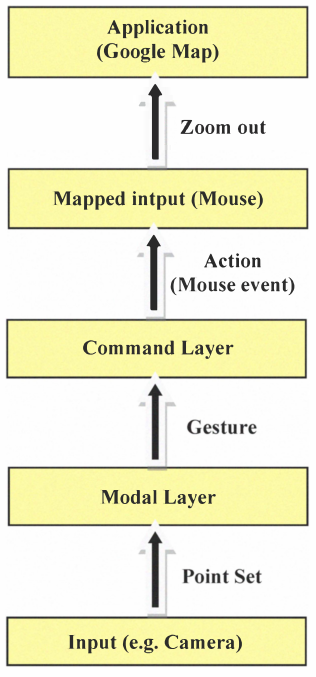
\includegraphics[scale=0.5]{gfx/mfi_modules_action}
    \caption{Módulos de MFI en acción.}
    \label{fig:mfi_action}
  \end{figure}
\end{center}

Otro factor de diseño importante es la capacidad de añadir nuevas modalidades. Es decir, el soporte que se brinda al desarrollador, desde el framework o plataforma, para agregar una nueva modalidad al sistema. En muchos casos, solo se considera un subconjunto de tecnologías particulares, en lugar de un subconjunto de modalidades en general. Por ejemplo, no es lo mismo un framework que permite el desarrollo de aplicaciones que hacen uso del \textsf{Novint Falcon}\footnote{Falcon de la compañía Novint, es un dispositivo que permite generar feedback háptico mediante la utilización de un sistema de servo-motores especialmente diseñado. Para mas información sobre el producto pueden visitar el sitio de  \href{http://www.novint.com/index.php/novintfalcon}{Novint}. Para conocer mas sobre la modalidad háptica pueden dirigirse al apéndice \ref{ch:mod_air}.} exclusivamente, que otro que posibilita el desarrollo de aplicaciones que hagan uso de la modalidad háptica en general(\eg, \emph{MIF}). En este punto ambos trabajos presentan buenas soluciones. En particular, en \emph{i*Chameleon} se distingue una etapa del ciclo de desarrollo, la de integración de driver de dispositivo (\emph{Device Driver Integration}), donde los ingenieros de dispositivos pueden desarrollar los módulos necesarios para conectarlos al sistema, los mismos incluso pueden ser re-utilizados, lo que avala técnicas como DRY y minimiza el grado de error.
\linebreak
Siguiendo con la división planteada, se revisan los aspectos de diseño en trabajos donde la atención está puesta en frameworks que brindan soluciones a problemas específicos  \ie, entornos educativos, ambientes inteligentes, dispositivos móviles, etc.
Entonces los siguientes aspectos serán de interés: re-usabilidad de componentes multimodales, extensibilidad del framework, orientado a ciclo de desarrollo y facilidad de uso. Estos, entre otros aspectos, son tratados por \citet{dumas2009multimodal}.

Aquí se destaca el enfoque de \citet{cutugno2012multimodal}, en dicho trabajo descentralizan el framework consiguiendo distribuir la lógica entre servidor y clientes \ie, estos últimos pueden procesar el mecanismo de fisión. Esta separación es lograda a través del uso de un archivo XML de configuración. Por medio de este archivo el desarrollador puede:
\begin{itemize}
\item
Especificar los eventos que pueden generar un cambio de estado.
\item
Indicar los comandos que el usuario puede disparar del lado cliente.
\item
Indicar cómo el usuario puede activar estos comandos a través de las modalidades.
\end{itemize}
De esta forma, este archivo representa una abstracción, que le permite al desarrollador indicar cuales comandos podrán ser lanzados y a través de que acciones multimodales, todo esto a través de claras etiquetas XML. Así el sistema brinda facilidad de uso y una posibilidad de re-usabilidad de componentes multimodales, la cual depende de la configuración XML del framework y la posibilidad de compartirla entre otras instancias del mismo. Si bien el trabajo de \citet{da2013learning} es un trabajo en progreso, tiene gran potencial para demostrar extensibilidad del framework multimodal y facilidad de uso, ya que estas plataformas de educación online son utilizadas en diferentes ámbitos por un gran conjunto de usuarios finales y no solo desarrolladores experimentados.
Finalmente, es notable el trabajo de \citet*{lo2013chameleon} ya que además de considerar a la plataforma necesaria junto al framework, los autores incluyen diversos aspectos, como técnicas que posibilitan re-utilizar interacciones multimodales entre distintas aplicaciones. También presentan un caso de desarrollo completo de una aplicación, haciendo énfasis en la clara separación de responsabilidades que brinda su herramienta, la cual es conseguida gracias al alto grado de modularización del framework; estos distintos componentes pueden asociarse claramente a los distintos roles involucrados en el desarrollo integral de una aplicación multimodal. De esta manera, es posible dividir exitosamente el trabajo entre los distintos profesionales que intervienen en el desarrollo, estos son: ingenieros de dispositivo, diseñadores de modalidad, programadores y diseñadores de interacción.

\subsection{Sobre la Plataforma Propuesta}
Teniendo en cuenta estos factores de diseño, la estrategia presentada en este trabajo presenta una arquitectura de componentes, similar a la propuesta por la W3C, la cual tendrá como objetivos definir claramente responsabilidades y facilitar tanto la extension de la plataforma como así también aspectos de escalabilidad de la misma. En cuanto al soporte para añadir nuevas modalidades, se aprovecha la separación de responsabilidades antes mencionada, introduciendo una etapa similar a la de integración de dispositivo de \emph{i*Chameleon} con el agregado de un protocolo de comunicación que permita facilitar la inserción de nuevo hardware.
También se tendrá en cuenta, lograr una plataforma fácil de usar por los desarrolladores de aplicaciones web. La posibilidad de conectar nuevas modalidades estará dada por los módulos desarrollados por los ingenieros de modalidades; como el desarrollo de los mismos no esta atado a un lenguaje en particular, la posibilidad de compartirlos para re-utilizarlos no será tan directa, aunque si se gana en flexibilidad. Por otra parte, se considerará brindar una clara separación en componentes, de los cuales se puedan etiquetar claramente las responsabilidades. Con respecto a la capacidad de extender la plataforma, en principio se plantea como para ser extendida ``a los extremos'', es decir que no solo se contempla el crecimiento a través de la conexión de nuevas modalidades sino también desde el lado cliente, por medio de lo que pueden ser diferentes módulos que agreguen capacidades ''extra'' en la interacción con la aplicación y con las nuevas señales que esta recibe (producidas por las modalidades).

\section{Comparación del Escenario Actual}
La tabla ~\ref{tab:estado_arte_tabla} compara algunas de las soluciones tratadas en este capítulo. Se considera: si se soporta un canal de entrada y salida para la modalidad, se aclara si es de propósito general o no y cual es el grado de soporte al desarrollo de aplicaciones web en particular.

%\begin{landscape}
\begin{sidewaystable}[p]
%  \begin{table}
%	  \begin{tabularx}{630pt}{p{4.8cm}|p{2.2cm}|p{2.2cm}|p{3.5cm}|p{3.4cm}|p{3.6cm}}
%	  \begin{tabularx}{600pt}{p{4.6cm}|p{2.2cm}|p{2.2cm}|p{2.4cm}|p{3.2cm}|p{3.6cm}}
 	  \begin{tabularx}{565pt}{p{4.4cm}|p{2.2cm}|p{2.2cm}|p{2cm}|p{3.2cm}|p{3.6cm}}
      \toprule[2pt]
	    \tableheadline{Trabajos - Propiedad} & 
	    \multicolumn{1}{p{2.2cm}}{Modalidad: Entrada} & 
	    \multicolumn{1}{p{2.2cm}}{Modalidad: Salida} & 
	    \multicolumn{1}{p{2cm}}{Ámbito de la solución} &
	    \multicolumn{1}{p{3.2cm}}{Orientado a ciclo de desarrollo MMI} & 
	    \multicolumn{1}{p{3.6cm}}{Soporte al desarrollo de aplicaciones web} \\ 
	    \midrule
	    Introduction to a Framework for Multi-modal and Tangible Interaction &
	    Si &
	    Limitada &
	    General &
	    No \footnote{Los casos negativos o de ausencia de alguna propiedad, se deben a no estar explícitamente indicados en los trabajos, todas las soluciones analizadas presentan buenas practicas de desarrollo de software. \label{fn:review_note_no}}&
	    Medio \\
	    \midrule
	    i*Chameleon &
	    Si & 
	    Si & 
	    General & 
	    Si & 
	    Medio \\
 	    \midrule
 	    An innovative framework to support multimodal interaction with Smart environments. &
      Si &
      Limitada &
      Smart Environments &
      Parcial \footnote{Arq. en componentes, clara separación de los mismos pero no hay aclaración en el trabajo sobre este aspecto. \label{fn:review_note_parcial}} &
      Bajo \\
 	    \midrule
   	  e-Learning Environment with Multimodal Interaction &
   	  Si & 
   	  No &
   	  Plataformas Educativas, accesibilidad &
   	  No \footref{fn:review_note_no} &
   	  Medio \\
 	    \midrule
  	  Multimodal Framework for Mobile Interaction &
  	  Si &
  	  No &
  	  Dispositivos Móviles &
  	  Parcial \footref{fn:review_note_parcial} & % 
  	  Medio \\
 	    \midrule
 	    A Framework for the Development of Distributed Interactive Applications &
 	    Posible &
 	    Posible &
 	    UI Multi-dispositivo &
 	    No \footref{fn:review_note_no}&
 	    Bajo \\
	    \bottomrule
	  \end{tabularx}
	  \caption{Escenario actual en soporte multimodal para aplicaciones.}
    \label{tab:estado_arte_tabla}
%	\end{table}
%\end{landscape}
\end{sidewaystable}
\pagebreak

\section{Resumen del Capítulo}\label{sec:estado_arte_summary}
Se han analizado seis trabajos que representan la vanguardia en cuanto a tecnologías para el desarrollo de aplicaciones multimodales. Los mismos fueron clasificados de acuerdo al formato y a la especificidad de la solución. Entre los trabajos revisados se encuentra también el análisis de un framework para el desarrollo de aplicaciones multi-dispositivo con interfaces de usuario migratorias; este trabajo se considera como transversal a los otros y puntualmente son de interés las soluciones arquitectónicas que brinda a un problema similar. 

También se destaca la plataforma propuesta por \citet*{lo2013chameleon} como la solución mas completa y de referencia para este trabajo. Luego se analizan algunos aspectos de diseño que deben sortear tecnologías de este estilo. Especificamente, se analiza: modularidad de la plataforma en relación a arquitecturas conceptuales como la de la W3C \citep{w3c:mmiarch}, facilidad para añadir nuevas modalidades, posibilidad de re-utilizar modalidades, extensibilidad, facilidad de uso para los desarrolladores y soporte para un ciclo de desarrollo. También se exponen las estrategias seleccionadas por la solución aquí propuesta. 

Finalmente se presenta un cuadro que aglomera algunas de las características mas importantes de los trabajos analizados.

% # FIN
%############################################################################ % Chapter 1

\cleardoublepage % Empty page before the start of the next part

%------------------------------------------------

\ctparttext{A continuación se exponen las características del medio al cual se agregará el soporte para las diferentes modalidades. Luego se esgrimirán los aspectos particulares que esta arquitectura propone y su relación con otras alternativas clásicas
.
En este trabajo, el ``medio'' es la Web como plataforma. Sobre la misma se construye la solución aquí propuesta; es entonces importante conocer las condiciones que este medio impone para comprender mejor la plataforma.

Al proponer una solución novedosa en determinados aspectos, fue necesario primero buscar algunos puntos de comparación en el desarrollo de plataformas multimodales. A continuación se analizan y comparan la arquitectura de \emph{Plusultra} con los trabajos de Dumas y la W3C.} 

\part{Aspectos Técnicos} % Segunda Parte

% Chapter 2 - Infraestructura

\chapter{Infraestructura} % Chapter title

\label{ch:infra} 

%----------------------------------------------------------------------------------------

% ### Introducción de capitulo

En los trabajos analizados en el capitulo \ref{ch:estado_arte}, las soluciones propuestas han necesitado algún conjunto mínimo de capas de abstracción, que les permita brindar el soporte para la conexión o el agregado de alguna modalidad especifica en un sistema particular.

El trabajo de \citet{dumas2009multimodal} presenta una arquitectura genérica para el desarrollo de aplicaciones multimodales, como se puede ver en la figura \ref{fig:arq_others_dumas}. Esta será una referencia importante en esta parte del documento.

En el presente capitulo se introducirán las decisiones de bajo nivel de la solución propuesta para la conexión de nuevas modalidades al contexto de una aplicación web, las mismas constituirán la plataforma denominada \emph{Plusultra}. 

Primero se describen las características generales de las aplicaciones web (clientes de la plataforma), para luego introducir las decisiones arquitectónicas. En el siguiente capitulo se completan los aspectos de desarrollo, añadiendo el modulo cliente (que corre en las aplicaciones web).
%Aquí se mostrará la estrategia seleccionada para desarrollar la plataforma.

\section{Características de las Aplicaciones Web} \label{sec:web_app_def}

El concepto de \emph{aplicación web} ha evolucionado desde sus inicios, con algunos pasos destacados como el surgimiento de AJAX en los 90s, que introdujo una nueva capa en el cliente mediante un conjunto de tecnologías con el fin de fragmentar la comunicación con el servidor, mejorando la experiencia de usuario; según indica \citet{garrett2005ajax}. Desde ese momento, las aplicaciones web fueron delegando, consistentemente, lógica de negocio hacia el cliente. 

En los últimos años, han surgido conceptos desde el ámbito académico como RIA (Rich Internet Applications) \citep{Fraternali2010}, que busca dar un marco conceptual a dicho movimiento. Por el lado de la industria, el desplazamiento hacia el cliente también es claro, librerías como Backbone.js \citep{ind:backbone} (desde el 2010), como una de las mas populares e inspiradoras para otros frameworks como Ember.js \citep{ind:ember} y Angular.js \citep{ind:angular}, han llevado el paradigma MVC fuera del servidor.

Por otra parte, el proyecto Node.js \citep{infra:nodejs}, a través de V8, permite la utilización de JavaScript del lado del servidor. Esta característica ha generado versatilidad en el software desarrollado, la misma puede observarse con proyectos como \emph{Browserify} \citep{infra:browserify} que posibilita la generación de módulos híbridos, capaces de correr en ambos extremos (cliente y servidor). Teniendo en cuenta esto, sumado a la ya conocida sólida presencia de JavaScript, como lenguaje estándar en el entorno del navegador, ha impulsado el ecosistema de desarrollo en JavaScript, posicionando a npm, como uno de los manejadores de paquetes mas populares hoy en día \citep{infra:npm-mods}. 

\subsection{Aspectos Particulares de las Aplicaciones Web Actuales}

Las aplicaciones web han evolucionado tomando formas similares a las de las aplicaciones de escritorio. Es decir, aplicaciones tipo single-page (SPA), con  múltiples componentes de interfaz de usuario que permitan la interacción con datos in-situ sin necesidad de refrescar o navegar a diferentes secciones.
Por \emph{single page applications} (SPA) o \emph{single page interface} (SPI)\citep{infra:spamanifesto} se hace referencia a aquellas aplicaciones web que cuentan con las siguientes características: minimizan la carga inicial de componentes a un request (\emph{single page load}), modularizan el contenido JavaScript (abstrayendo las llamadas AJAX con el servidor), tienen capacidad de manejar ruteo y la historia del navegador, soporte de templates \emph{client-side}, comunicación bidireccional (\emph{real-time}) con el servidor y capacidad de usar almacenamiento local en el cliente. 

El concepto de RIA (\emph{Rich Internet Applications}) define estos nuevos tipos de aplicaciones. Es decir, el cambio que hubo desde compartir contenido estático hasta el dinamismo actual.
Con el fin de expandir las características definidas a través del termino \emph{RIA} y buscando describir mas estrictamente el escenario donde serán incluidas la capacidad de usar múltiples modalidades, se define el siguiente listado de características que hacen a una aplicación web actual:

\begin{itemize}
\item \textbf{Aplicaciones inherentemente distribuidas}; de acuerdo al paradigma de comunicaciones cliente-servidor, aún vigente en la web, las aplicaciones se conectan al servidor para obtener algo y realizar alguna tarea, el servidor luego puede centralizar resultados. En la web, ocurre algo similar, las aplicaciones web, a través de los agentes de usuario, descargan toda la aplicación, incluso algún conjunto de datos básico; esto le permite al usuario interactuar con la aplicación en su completitud e incluso de forma ''offline'' si se adecuan algunos parámetros.

\item \textbf{Aplicaciones inherentemente multiplataforma}; luego del surgimiento de la \emph{web 2.0}, se consolida la web como plataforma (\emph{Web as a plataform}), este concepto se apoya en la multiplicidad de servicios que la web ofrece o que una aplicación desarrollada para este ecosistema puede consumir, de acuerdo a \citet{infra:html5}. Estos servicios, son ofrecidos a través de vínculos nativos, por el navegador del usuario. Las aplicaciones son codificadas en lenguajes estándares, que corren dentro del ambiente provisto por el navegador.

\item \textbf{Clientes ``pesados'' con características de aplicaciones de escritorio}; la lógica de aplicación ya no se encuentra totalmente en el servidor. El servidor provee funciones de centralización (\ie  autenticación) o recursos a través de \emph{APIs} (\ie  REST); pero la manipulación y el tratado de los mismos ocurre del lado del cliente.

\item \textbf{APIs estándar para consumo de características nativas de hardware}; a través de la W3C, se busca expandir la web en múltiples direcciones. En \citep{infra:html5} se listan varios de estos tópicos. Por ejemplo, se destaca, la API de Vibración \citep{infra:vibration} o la especificación para el acceso a eventos táctil \citep{infra:touch}; las mismas definen como utilizar diferentes capacidades de interacción.

\item \textbf{Adaptabilidad}; mediante estrategias como \emph{responsive-design} es posible no solo adaptar contenido de acuerdo a la pantalla del dispositivo, si no también, a las características disponibles de cada uno. Se desarrolla buscando una mejora progresiva. Entre otras ventajas, esto permite mantener una única base de código en lugar de diseñar diferentes aplicaciones, tanto para escritorio como para dispositivos móviles.

\marginpar{Socket.io y WS, son proyectos open source, desarrollados en JavaScript, que implementan el protocolo WebSocket. Si bien difieren en como lo implementan, ambas 
librerías permiten crear clientes y servidores de WebSockets.}

\item \textbf{Bidireccional en el inicio de la conversación}; \emph{Web Sockets} es otra especificación de la W3C \citep{infra:websockets}, con implementaciones concretas utilizadas por la industria, como \href{http://socket.io/}{Socket.io} o \href{http://einaros.github.io/ws/}{WS}, entre otras; permiten la comunicación bidireccional entre cliente y servidor y el ``inicio de la conversación'' por parte de las aplicaciones web. Esto posibilita un escenario con características de \emph{tiempo-real}.
\end{itemize}

\section{Arquitectura Propuesta} \label{sec:arq_ours}
Teniendo en cuenta el escenario planteado, insertar de forma genérica una nueva modalidad implica algunos desafíos técnicos. A continuación se describe la estrategia elegida y su fundamentación. La misma se compone, a grandes rasgos, de tres partes; dos \emph{APIs}, una para el navegador como una dependencia mas de la aplicación web y la otra para conectar la nueva modalidad al entorno web; el componente restante es una pasarela de mensajes. Es el componente que sera descrito en este capitulo, los otros dos serán tratados mas adelante.

% FIGURA DE COMPONENTES ARQ - single app
\begin{center}
  \begin{figure}[h]
    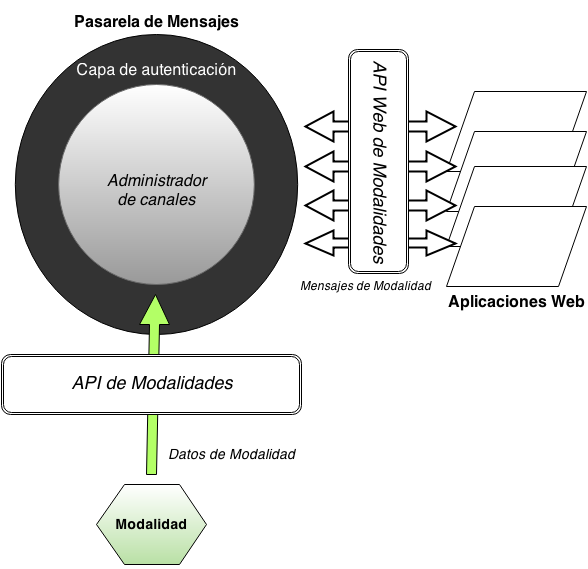
\includegraphics[scale=1,width=\textwidth]{gfx/arq_simple_es}
    \caption{Componentes de arquitectura para una aplicación web}
    \label{fig:arq_ours_single_app}
  \end{figure}
\end{center}

\subsection{Pasarela de Mensajes: Introducción} \label{sec:arq_ours_intro}
En la figura \ref{fig:arq_ours_single_app} se puede observar de manera rápida la arquitectura del sistema. En esta sección se pondrá el foco sobre el \emph{Message Gateway} o \emph{Pasarela de Mensajes}; de ahora en mas se usará PM para referirse a la misma con el fin de abreviar.
En la construcción de la PM se tuvo en cuenta un modelo de capas, con el \emph{Channels Manager} o \emph{Administrador de canales} como núcleo y único componente requerido para su funcionamiento. El resto de las capas agrega funcionalidades, de manera muy similar a la de un \emph{middleware}. Es decir, interceptan los mensajes, los utilizan como entrada para ampliar el contexto, validar el pedido o cualquier otra tarea que pueda hacerse con los datos del mensaje; luego de realizada dicha tarea, le pasan el mensaje al siguiente nivel de profundidad hasta llegar al núcleo.

El núcleo, a través de una base de datos en memoria, mantiene los canales activos de comunicación. Un canal equivale a una aplicación. Los canales pueden ser multiplexados, es decir, usando un canal, podemos fragmentarlo y generar sub-canales en caso de ser necesario. 
El núcleo, implementa un patrón similar al de \emph{Publishers/Subscribers}, entonces, de forma simple, cuando recibe un mensaje, chequea el canal por el cual debe retransmitirlo hacia todos los clientes suscritos al mismo. Como se ha mencionado antes, es valido visualizar una cardinalidad 1 a 1 entre canales y aplicaciones. 

Por otra parte, una aplicación puede tener \emph{N} clientes. Cada cliente conectado a la aplicación, es automáticamente suscrito a su correspondiente canal, a través de la API provista al navegador (usando el módulo \emph{Gyes} que veremos en el próximo capitulo). De manera similar, la modalidad, a través de la interfaz provista para las mismas se conectará al canal de aplicación que le corresponda. Ya sea una persona (desarrollador) o un equipo de trabajo multimodal, deberán tener acceso al token de acceso por aplicación. Este token podría ser accedido mediante alguna aplicación de registro a la plataforma como servicio o podría ser simplemente generado y distribuido internamente en el grupo de trabajo, si se toma la decisión de hostear de forma autónoma una instancia de la plataforma. 

De cualquier manera, se genera un puente entre modalidad y aplicaciones cliente, lo que equivale a decir que es posible intercambiar mensajes bidireccionalmente entre aplicaciones ``cliente'' y modalidades conectadas a la aplicación. Por lo que no solo los clientes se ven afectados por la señal generada por la modalidad, si no que ellos también pueden modificar, por ejemplo, la configuración de la modalidad en tiempo-real. La cual es una característica con la que muy pocos sistemas multimodales cuentan.

\marginpar{PaaS o en español, plataforma como servicio, hace referencia a una plataforma en la nube que brinda una solución que puede ser aplicada por el consumidor como una capa mas a su sistema, abstrayéndolo de diferentes cuestiones relacionadas al hardware y brindándole capacidades de escalabilidad.}
Otra capa importante pensando en la plataforma como PaaS (\emph{Platform as a Service}), y que esta provista en el sistema de forma inicial, es la de autenticación (\emph{Authentication Layer}). La forma de autenticar clientes es algo simple, pero efectiva para el caso. Se basa en una estrategia tipo ``algo que posea'' el cliente. En este caso, al registrar una aplicación web que usará esta plataforma, la misma recibirá un \emph{token}. Tanto el desarrollador de modalidad (si es que lo hay), como el desarrollador de la aplicación web, comparten este token. El sistema registra a la aplicación con un token y un canal. Cabe destacar que en este aspecto puntual, por aplicación se refiere tanto a las modalidades usadas como a los clientes web (son todos ``parte de'').

Al llegar un mensaje nuevo, tanto por parte de un cliente como de una modalidad, esta capa lo intercepta, toma el token que viene con el mensaje, y lo valida. Si es positiva, el mensaje continua a la siguiente capa, y se cachea el token para mejorar la performance en futuros mensajes. Si no es valido, el mensaje es desechado y no continua. Este proceso se describe aquí de manera rápida, porque el foco, por el momento no esta puesto en la seguridad del sistema, pero se cree que es un mecanismo que junto con otras previsiones puede garantizar autenticidad sin producir demasiado \emph{overhead} en la comunicación.

\subsection{Pasarela de Mensajes: Diseño} \label{sec:arq_ours_design}
La pasarela de mensajes \emph{Plusultra}, esta implementada usando un esquema de interacción distribuida tipo \emph{publish/subscriber}, ver figura \ref{fig:infra_pubsub}. Se decidió utilizar un esquema de comunicación basado en eventos para favorecer a los dispositivos de modalidad, los principales productores del sistema. Los dispositivos de modalidad pueden ser clasificados como reconocedores, sintetizadores o ambos. De cualquier forma, estos se comunicarán a través de eventos, \eg generando uno luego de reconocer un gesto (patrón) o recibiendo un evento que señalice la ocurrencia de una fisión, dando lugar a una posible acción de sintetizado.

% FIGURA DE PUBSUB
\begin{center}
  \begin{figure}[h]
    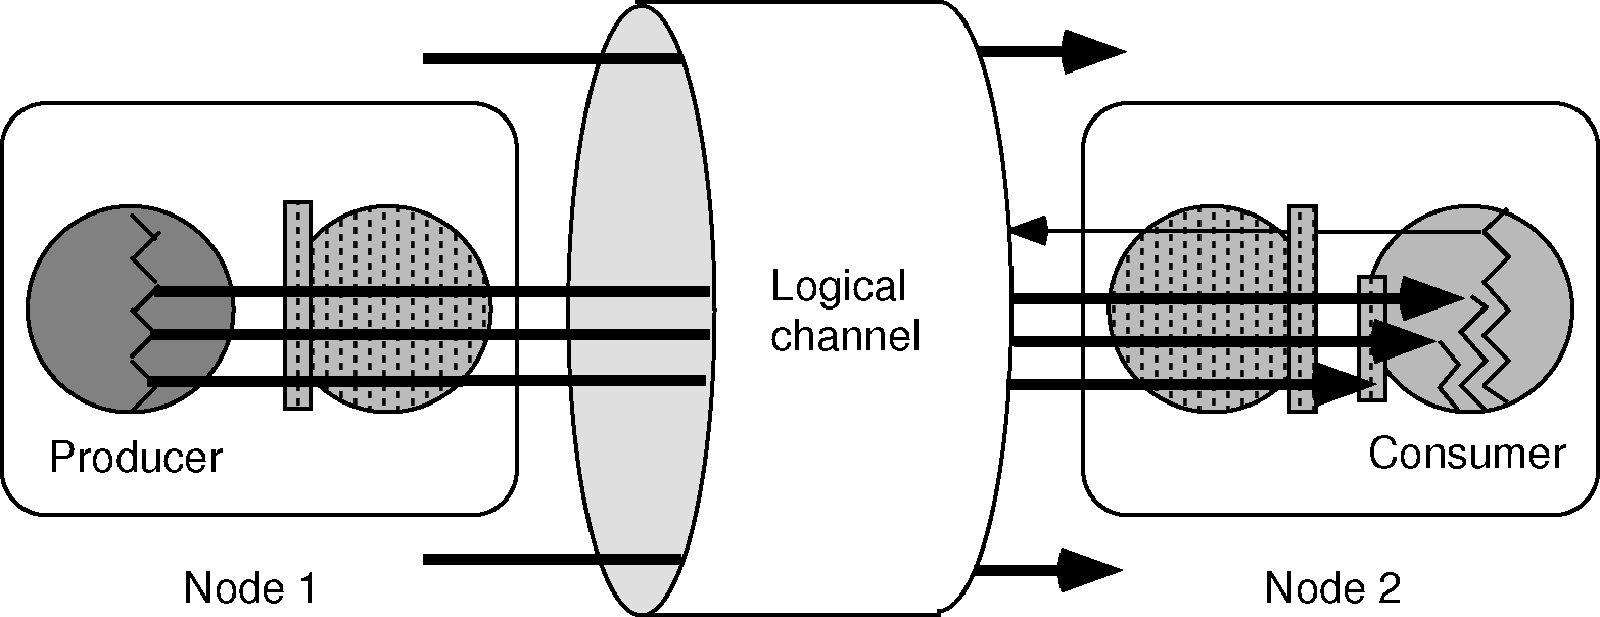
\includegraphics[scale=1,width=\textwidth]{gfx/pubsub}
    \caption{El paradigma de interacción Publishers/Subscribers, de acuerdo a \citet{Kermarrec2003}.}
    \label{fig:infra_pubsub}
  \end{figure}
\end{center}

Los eventos pueden ser mensajes en texto plano o con algún formato, como JSON en este caso. Los mismos encapsulan un protocolo de comunicación que se definirá junto al modulo cliente \emph{Gyes}, mas adelante. 

\marginpar{Redis, es un sistema open source, que permite almacenamiento y cacheo de estructuras \emph{clave-valor}. Es también conocido como un servidor para estructuras de datos. Para mas información visitar: \href{http://redis.io/}{redis.io}}
La información sobre canales y aplicaciones activas es almacenada utilizando algún sistema de base de datos en memoria, en la implementación actual se utiliza \textbf{Redis} (configurado especialmente para no persistir datos), esto permite un acceso rápido a la información de una aplicación y ayuda a perfilar a la plataforma como un sistema de intercambio de mensajes volátil, es decir, esto no es una base de datos ni una cola de mensajes. 

Cada instancia de la pasarela funciona como un modulo \emph{productor/consumidor} distribuido. Esto permite ver al sistema en general como un motor de notificación de eventos distribuido en un conjunto de procesos y servidores, compartiendo diferentes bases de datos en memoria. Esta visión se corresponde con la del sistema funcionando como un PaaS, aunque también puede correr \emph{standalone}, es decir, como una unidad de trabajo particular. Esta forma de ver al sistema corresponde con una arquitectura \emph{publishers/subscribers} centralizada, muy similar a una cola de mensajes. 

Las principales ventajas de implementar a \emph{Plusultra} como un sistema de notificación \emph{publish/subscriber} radican en tres cualidades, de acuerdo con \citet{Kermarrec2003}:
\begin{itemize}
\item \textbf{Desacoplamiento en tiempo}; las partes que interactúan, dispositivos de modalidad y aplicaciones, no necesitan estar conectadas al mismo tiempo para comunicarse. Los dispositivos de modalidad son independientes al número de clientes conectados y viceversa. La importancia radica en el momento, esto es, si se produce una señal entonces puedo captarla y hacer algo; ``si ocurrió una señal en el pasado no me interesa''.

\item \textbf{Desacoplamiento en espacio}; este desacople se produce entre aplicaciones y dispositivos de modalidad e implica que no es necesario que estos entes se conozcan entre ellos para funcionar. Las dispositivos envían señales, en forma de eventos, hacia la plataforma y continúan su trabajo. Por otra parte, los clientes, es decir las aplicaciones web, cuando detectan una nueva fusión (que pudo haberse producido) por una señal de una modalidad, pueden ejecutar un \emph{callback} asociado en ese momento. 

\item \textbf{Desacoplamiento en sincronización}; No ocurre ningún tipo de bloqueo entre dispositivos de modalidad y clientes web. Cuando una señal es reconocida y un evento es disparado, el driver del dispositivo nunca esperará por una respuesta para ``continuar''. De forma similar, cuando algo ocurre y se debe señalizar a una aplicación, este evento particular generará la ejecución de un \emph{callback} en el cliente; es decir, éste nunca se detuvo a esperar por la ocurrencia de dicho evento.

\end{itemize}

La plataforma fue diseñada teniendo en cuentas estas características. Mas aun, un sistema desarrollado teniendo en cuenta estos items tendrá facilidades al momento de escalar \citep{Kermarrec2003}.

Los desafíos o posibles inconvenientes a los que puede verse afectado un sistema de notificaciones de este tipo se encuentran en el hardware y plataforma sobre la que corran, así como también de las posibles limitaciones en la topología y protocolos de comunicación usados. Por ejemplo, el sistema puede verse beneficiado si se utiliza un protocolo de comunicación probabilístico en lugar de uno diseñado para \emph{WAN} como RMTP, que genera \emph{overhead} debido a la gran cantidad de mensajes de confirmación que ocurrirían \citep{Kermarrec2003}.
La extensión y consolidación de esta \emph{Plusultra} como PaaS queda fuera del alcance de este trabajo y sería posible analizarla solo con mas tiempo y en condiciones diferentes.

\subsection{Pasarela de Mensajes: Implementación} \label{sec:arq_ours_code}
Para implementar la pasarela se ha decidido utilizar \textbf{Node.js}. Esta tecnología, comprende a un entorno de desarrollo multi-plataforma (gracias al motor V8 en el que corre), orientado a I/O y con una arquitectura basada en eventos, lo que lo convierte en una herramienta favorable para desarrollar servicios o aplicaciones orientadas a \linebreak{\emph{networking}}, como es el caso de la plataforma aquí propuesta; donde el foco esta puesto en las comunicaciones y no en el procesamiento.
Otra ventajas de usar Node.js, es que se mantiene un mismo lenguaje para el código del proyecto: JavaScript. Haciendo mas fácil pasar de una tarea a otra. Por ejemplo cambiar de contexto, al desarrollar un modulo cliente y luego volver a la plataforma.

\section{Comparación con la Arquitectura Clásica} \label{sec:arq_others}
Se considera como \emph{arquitectura clásica} para un sistema con interacciones multimodales a la definida por \citet{dumas2009multimodal}. En dicho trabajo, los autores abstraen las características genéricas que un sistema multimodal debería poseer, definen componentes arquitectónicos fundamentales. 

% FIGURA DE COMPONENTES ARQ CLASICOS - Dumas
\begin{center}
  \begin{figure}[h]
    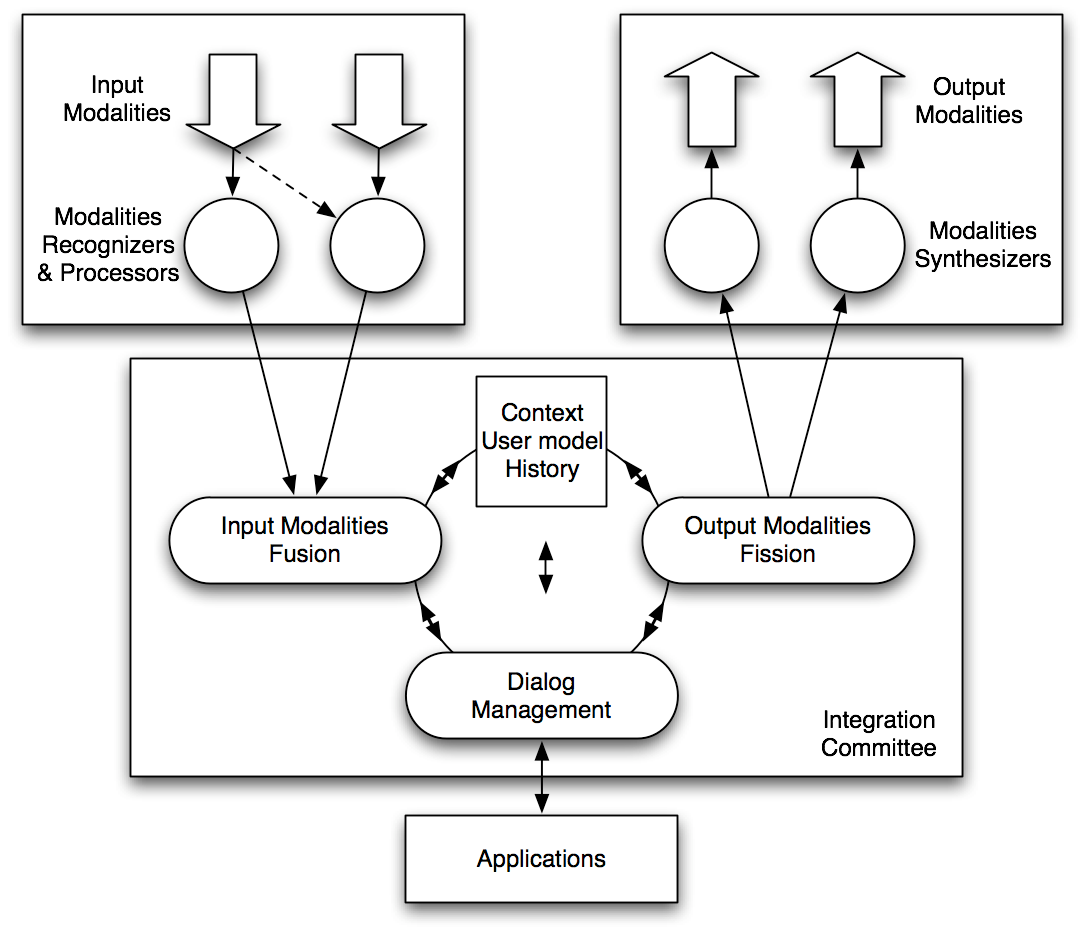
\includegraphics[scale=1,width=\textwidth]{gfx/arq_dumas}
    \caption{La arquitectura de un sistema multimodal clásico por  \citet{dumas2009multimodal}.}
    \label{fig:arq_others_dumas}
  \end{figure}
\end{center}

En la figura \ref{fig:arq_others_dumas} se pueden observar los principales componentes, el \emph{comité de integración} con sus sub-componentes y las modalidades con los correspondientes, \emph{reconocedores}, \emph{pre-procesadores} y \emph{sintetizadores} entre otros posibles filtros.

Este es un esquema claro en cuanto a la división de responsabilidades. La arquitectura propuesta en este capitulo se concentra en la forma de interconectar las modalidades, la implementación realizada del \textbf{comité de integración} será analizada en el próximo capitulo.
De acuerdo a las características antes mencionadas, la arquitectura debe ser capaz de insertarse en un ambiente distribuido. Es decir, debe ser capaz de conectar de una forma clara y efectiva modalidades (entrada y salida) con múltiples clientes de una aplicación web, en tiempo real. Para eso, como ya se ha mencionado, se utiliza un sistema de interconexión basado en eventos. Entones, re-interpretando la arquitectura clásica, el diseño de la solución propuesta se ve en la figura \ref{fig:arq_dumas_plusultra}.

% FIGURA DE COMPONENTES ARQ CLASICOS - Dumas + Plusultra
\begin{center}
  \begin{figure}[h]
    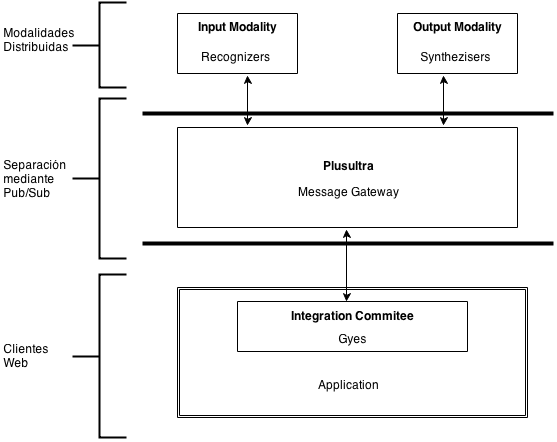
\includegraphics[scale=1,width=\textwidth]{gfx/Dumas_Plusultra}
    \caption{La arquitectura propuesta en este trabajo.}
    \label{fig:arq_dumas_plusultra}
  \end{figure}
\end{center}

La \emph{pasarela de mensajes}, se convierte en un aspecto central, que permite mantener la separación de responsabilidades original de la aplicación y a la vez adaptarse al contexto de una aplicación web.

Ese diseño brinda otra ventaja, importante si se piensa a la \emph{plataforma como servicio}, se trata de la capacidad para escalar horizontalmente, como se ha mencionado en la sección \ref{sec:arq_ours_design}. En el siguiente gráfico \ref{fig:ours_single_app_scalable_scenario} se muestra un hipotético escenario escalable. Esta es solo una configuración posible para conseguir escalabilidad, utiliza un balanceador de carga como una dependencia externa (\ie nginx); otra alternativa podría desechar la necesidad de agregar otro componente mediante el desarrollo de una nueva capa de ``middleware'' que auto-balancee la carga y distribuya a otro cliente, de los posibles instanciados por el usuario de la plataforma. Hay mas alternativas para explorar y queda abierto (escapando a los objetivos del presente trabajo), en el campo de PaaS o de servicios sobre Internet en general, elegir y probar los mejores caminos.

% FIGURA DE COMPONENTES ARQ - our, scalable
\begin{center}
  \begin{figure}[h]
    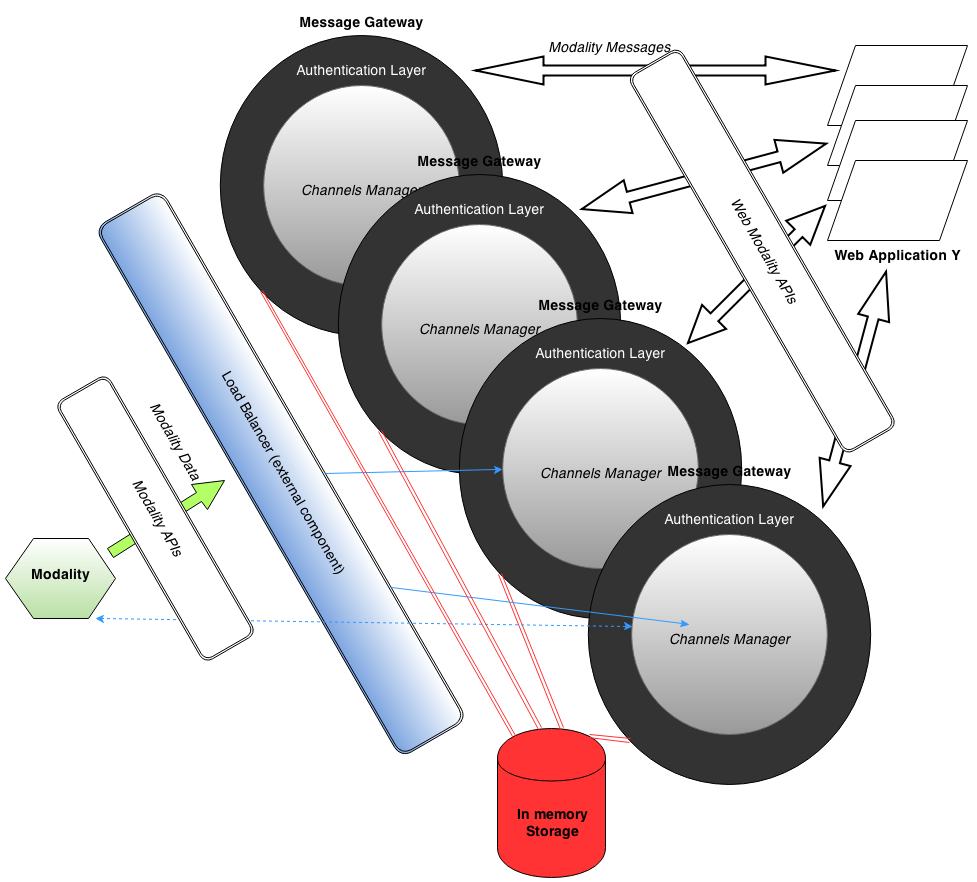
\includegraphics[scale=1,width=\textwidth]{gfx/arq_scalable}
    \caption{Componentes de arquitectura en un escenario escalable, múltiples PMs.}
    \label{fig:ours_single_app_scalable_scenario}
  \end{figure}
\end{center}


\section{Comparación con la Arquitectura Propuesta por la W3C} \label{sec:arq_others_w3c}
En \citet{w3c:mmiarch}, se propone una arquitectura similar a la denominada ``clásica''. Dentro del \emph{Runtime Framework}, donde se definen muchos aspectos técnicos y que esta delegado a quien implemente la arquitectura se define un \emph{Interaction Manager}(administrador de interacción) o IM, que debe recibir todos los eventos generados por los diferentes \emph{Modality Components}(componentes de modalidad) o MC; allí se define la interacción con el componente. Algo similar a los componentes de fisión y fusión de la arquitectura clásica, solo que aquí se encuentran distribuidos. El modulo IM es similar a la pasarela de mensajes de la estrategia propuesta. La diferencia radica, en parte, en la fuerte orientación a eventos y a trabajar como máquina de estados por parte del IM. En cambio el componente PM, en un principio, esta orientado a trabajar transmitiendo datos en ``crudo'' por parte de las modalidades y no eventos. Aunque esto puede modificarse, añadiendo algún tipo de pre-procesador de los datos generados por la modalidad. Esto depende del ingeniero de modalidad.

Las modalidades se definen usando algún tipo de lenguaje de marcado (\ie CCXML, SCXML, HTML, entre otros). Otra diferencia importante entre el sistema propuesto por la W3C y el del presente trabajo, es la API que conecta el IM con los diferentes MC. Es la sección menos flexible del documento \citet{w3c:mmiarch}. En ella se definen cuestiones tales como activación y detención de la modalidad, acciones previas a recibir un mensaje, inicio y fin de la conversación. Esta API le da fuerza al modelo de máquina de estados. 

En este trabajo no se considera un modelo de maquina de estado porque en un principio se busca favorecer al máximo, o lo que es lo mismo, minimizar cualquier tipo de obstactulo en la transmisión de datos ``crudos''. Por otra parte, la estrategia aquí presentada, mueve los componentes de fisión y fusión a los clientes y le entrega dicha responsabilidad al desarrollador de la aplicación para que fusione con libertad el contexto de la aplicación que esta desarrollando con las modalidades disponibles. Se cree que de esta manera se puede explotar el uso de las modalidades.

En el gráfico \ref{fig:arq_others_w3c} se muestra la arquitectura propuesta por la W3C antes mencionada.
% FIGURA DE COMPONENTES ARQ - others, w3c
\begin{center}
  \begin{figure}[h!]
    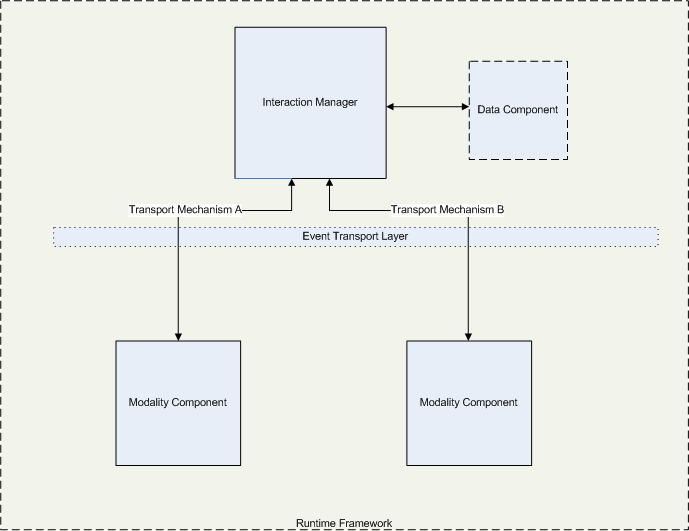
\includegraphics[scale=1,width=\textwidth]{gfx/w3c_RevisedArchDiagram}
    \caption{Arquitectura de la W3C en tiempo de ejecución}
    \label{fig:arq_others_w3c}
  \end{figure}
\end{center}
\large

\hfill
\vfill

\section{Resumen del Capítulo} \label{sec:infra_summary}
En este capítulo se ha mostrado la estrategia elegida en la creación de la arquitectura necesaria para poder expandir las capacidades de las aplicaciones web actuales con el uso de nuevas modalidades. Se han detallado características particulares al ambiente de las aplicaciones web y que han influido en las decisiones tomadas para desarrollar dicha arquitectura. A su vez, se ha comparado el trabajo realizado con otras soluciones conocidas, como son el modelo presentado por \citet{dumas2009multimodal} y el trabajo del grupo de MMI \citet{w3c:mmiarch}

Mas adelante, se completara la arquitectura, definiendo la implementación elegida para el ``núcleo'' de la misma, como son los componentes de \emph{fusión} y \emph{fisión}; con el fin de mantener la claridad se ha decidido analizarlos por separado.


%############################################################################ % Chapter 2

\cleardoublepage % Empty page before the start of the next part

% Chapter 3 - APIs, enlace con las modalidades

\chapter{Enlace con las modalidades} % Chapter title

\label{ch:enlace} 

%----------------------------------------------------------------------------------------

% ### Introducción de capítulo

 
\section{Arquitectura Propuesta} \label{sec:enlace_overview}
%Primer vistazo general de los ''endpoints'' del sistema, que conectamos? como se consume?
A grandes rasgos, los puntos de entrada a la plataforma \emph{Plusultra} introducida en el capítulo anterior, estarán ubicados en dos lugares diferentes:

\begin{itemize}
\item \textbf{Clientes Web}; aquí también reside la lógica de la aplicación. En conjunto crean una experiencia multimodal en la web. Dentro de los clientes web, podemos encontrar capacidades extra que pueden ser usadas a su vez como modalidades (\ie ~un cliente corriendo en un smartphone puede tener acceso a sensores, que a su vez, pueden ser usados como reconocedores). Mas adelante en este capítulo, se analizará esta situación.
\item \textbf{Dispositivos de modalidad}; se refiere a todos aquellos dispositivos especialmente dedicados a reconocer o sintetizar una modalidad, \eg~ Falcon de Novint o Leap Motion, por mencionar algunos.
\end{itemize}

Para conectar estos puntos de entrada, se construyo un modulo de acceso que puede ser consumido por igual tanto del lado del cliente como del servidor o \emph{standalone} (dispositivos de modalidad). Ademas se ha desarrollado una primera versión de un protocolo de comunicación que acompaña dicha interfaz de comunicación. Este protocolo abre el camino a otros desarrolladores para que puedan diseñar soluciones utilizando diferentes lenguajes. 
En el mismo se describe los mensajes utilizados para un enlace efectivo con la plataforma \emph{Plusultra}. De esta manera, siguiendo a este protocolo versionado, la API puede portarse a otros lenguajes de programación extendiendo así el alcance y uso de la plataforma.

\subsection{Modulo Híbrido Cliente/Servidor}
Prácticamente todo el desarrollo de este trabajo se ha llevado a cabo utilizando el lenguaje JavaScript. Dado que se busca expandir la capacidad actual de comunicación de las aplicaciones web, es lógico basar la mayor parte de la base de código en dicho lenguaje. Usando la plataforma Node.js, es posible correr JavaScript del lado del servidor también, haciéndolo ubicuo en múltiples escenarios. Teniendo en cuenta estas capacidades, se decidió desarrollar un modulo que pueda aprovechar estos aspectos y ser de utilidad en diversas circunstancias o casos de uso.
 
De esta forma se introduce el módulo \emph{Gyes}. A través de este componente es posible conectarse al sistema, transmitir datos de modalidades, crear nuevas modalidades, crear interpretaciones, capturar salidas del sistema de fisión; por nombrar los casos mas importantes. 

\subsection{Vista General}
%Grafico que muestre los componentes introducidos antes y las nuevas interfaces.
El modulo \emph{Gyes} permite realizar diferentes tareas, las cuales tienen como finalidad interactuar con la plataforma \emph{Plusultra} y por consiguiente con el resto de los actores de la aplicación, es decir, con el contexto entero de la aplicación web.
El siguiente gráfico \ref{fig:arq_ours_gyes_action} simplifica una de las principales actividades, utilizar una modalidad como reconocedora de algún tipo de señal para luego propagarla en la aplicación, mediante la plataforma. 

% FIGURA DE GYES en accion
\begin{center}
  \begin{figure}[h]
    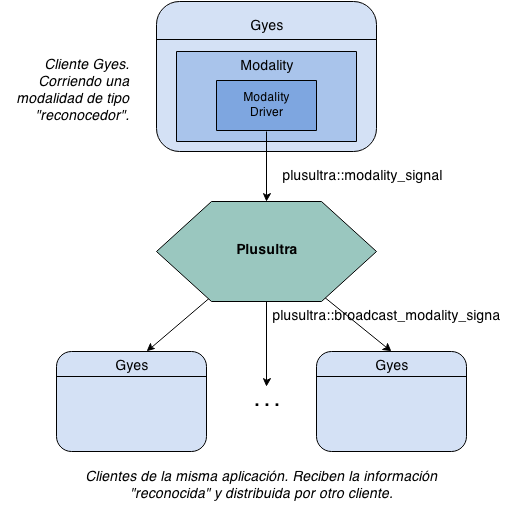
\includegraphics[scale=0.7]{gfx/gyes_action}
    \caption{Modulo Gyes en acción: transmitiendo señales}
    \label{fig:arq_ours_gyes_action}
  \end{figure}
\end{center}

\section{Descripción de la Interfaz del Modulo} \label{sec:enlace_api}
% detalles de la interfaz
En la figura \ref{fig:arq_ours_gyes} se observa de manera directa los principales componentes del modulo de acceso al sistema. Luego extenderemos esta visión a la interacción que ocurre con la plataforma.
A continuación se describirán las interfaces de los componentes junto a una breve introducción a la primer version del protocolo de comunicación entre \emph{Plusultra} y \emph{Gyes}.

% FIGURA DE COMPONENTES GYES
\begin{center}
  \begin{figure}[h]
    \centering
    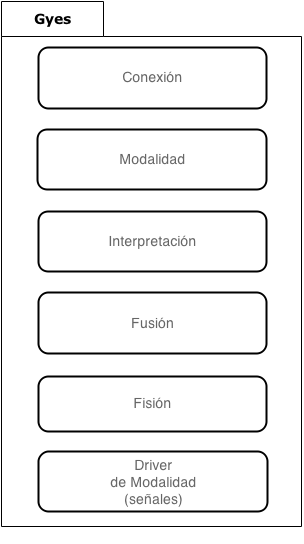
\includegraphics[scale=0.7]{gfx/gyes}
    \caption{Principales componentes del modulo Gyes}
    \label{fig:arq_ours_gyes}
  \end{figure}
\end{center}

\subsection{Componente de Conexión}

Es el componente principal. Desde aquí no solo accedemos a la plataforma si no también al resto de los componentes. 

La función principal es proveer una forma de conectar, tanto para modalidades como clientes a \emph{Plusultra}.
\\

\underline{\textsf{Constructor:}}\\
\begin{lstlisting}
Gyes( appKey, uri, opts )
\end{lstlisting}
Crea una nueva instancia del módulo \emph{Gyes}. Automáticamente inicia una conexión con la plataforma \emph{Plusultra}. 

\underline{\textsf{Principales métodos:}}\\
\begin{itemize}
\item[]
\begin{lstlisting}
gyes::authenticate( appKey )
\end{lstlisting}
Una vez creada la instancia, necesitamos autenticar nuestra aplicación. Para eso el desarrollador web debe contar con una llave, previamente generada, por ejemplo usando algún servicio donde registre la aplicación y la cantidad de instancias a consumir de la plataforma.
\\

\emph{Plusultra} es una plataforma que ha sido diseñada para ser fácilmente escalable a un modelo de PAAS (\emph{Platform as a Service}), de esta forma, múltiples instancias del módulo de plataforma pueden servir a diferentes aplicaciones. Por eso es necesario que cada aplicación posea una llave que la distinga.

\item[]
\begin{lstlisting}
gyes::addModality( aModality )
\end{lstlisting}
Permite agregar una nueva modalidad al sistema. Esto es útil para indicar que determinado cliente cuenta con una modalidad particular la cual, al estar ``agregada'' a la plataforma, puede compartir la información que genera.
\end{itemize}

\subsection{Componente de Modalidad}
%diagrama de secuencia, conexion, fusion/fision

Este módulo permite crear y agregar nuevas modalidades al sistema. Dada la naturaleza variada de las mismas, se decidió separar comportamiento de representación/identificación. El comportamiento esta definido por los drivers, aquí especificamos una representación. Dentro de una aplicación, pueden conectarse mas de una modalidad y por ahora, una modalidad puede usar un driver.
\\

\underline{\textsf{Constructor:}}\\
\begin{lstlisting}
Gyes::Modality( name, type, opts )
\end{lstlisting}
Permite crear un nuevo objeto que representa a una modalidad, la cual podrá ser agregada al sistema. Recibe un nombre (\emph{name}), tipo (\emph{type}), de acuerdo a si es de entrada/salida o ambos y luego opciones (\emph{opts}) particulares para compatibilidad a futuro.
\\

\underline{\textsf{Principales Métodos:}}\\
\begin{itemize}
\item[]
\begin{lstlisting}
modality::use( modalityDriver )
\end{lstlisting}
Conecta una instancia de modalidad con una instancia de driver.
\end{itemize}

\subsection{Componente de Fusión Distribuida}

Permite controlar el motor de fusión de manera programable. Este componente captura \emph{señales} que pueden ser generadas por modalidades o por eventos de la aplicación.
\\

\underline{\textsf{Constructor:}}\\
\begin{lstlisting}
Gyes::Fusion( opts )
\end{lstlisting}
Genera una nueva instancia del motor de fusión. 
\\

\underline{\textsf{Principales métodos:}}\\
\begin{itemize}
\item[]
\begin{lstlisting}
fusion::fuse( anInterpretation )
\end{lstlisting}
Detecta un determinado conjunto de señales, definidos por una interpretación. Cuando dicha interpretación ocurre, puede distribuir esta información entre todos los clientes y comenzar el proceso de activar al sistema de fisión.
\\

La captura de señales se produce manteniendo una ventana de tiempo, donde la misma se actualiza (extiende) cada vez que ocurre un evento que pertenezca a una interpretación. Esto ocurre de forma independiente y distribuida entre todos de la aplicación. Es decir, cada uno cuenta con un motor de fusión. Para que esto funcione, las señales deben ser distribuidas, usando la plataforma, en tiempo real.
\end{itemize}

\subsection{Componente de Fisión Distribuida}

Brinda acceso al sistema de fisión. El desarrollador web, encuentra en este componente un ``punto de salida'' de la plataforma, donde puede conectar la lógica de la aplicación web mientras consume información generada por las distintas señales que recorren el sistema.
\\

\underline{\textsf{Constructor:}}\\
\begin{lstlisting}
Gyes::Fission( opts )
\end{lstlisting}
Genera una nueva instancia del motor de fisión.
\\

\underline{\textsf{Principales Métodos:}}\\
\begin{itemize}
\item[]
\begin{lstlisting}
fission::on( interpretationName, callbackFn )
\end{lstlisting}
El sistema de fisión permite al desarrollador conectar la ocurrencia, asincrónica, de una interpretación con código que afecte a la lógica de negocios de la aplicación.
\end{itemize}

\subsection{Componente de Interpretación}

En los componentes anteriores se menciono el concepto de \emph{interpretación}, aquí se muestra su interfaz y lo que representa.

Este componente permite agrupar un conjunto determinado de señales en un único objeto.
Una interpretación puede representar la conjunción de diferentes modalidades en un único evento.
Las interpretaciones son usadas por el motor de fusión para detectar la ocurrencia de dichas señales e interpretarlas como un único evento alertando al resto de los componentes del sistema sobre dicha ocurrencia.
\\

\underline{\textsf{Constructor:}}
\begin{lstlisting}
Gyes::Interpretation( eventsList )
\end{lstlisting}
Genera una nueva instancia de interpretación. Recibe una lista de señales la cual servirá para organizar al sistema de fusión en el escaneo y detección de ocurrencias de interpretaciones.
\\

\underline{\textsf{Principales Métodos:}}\\
\begin{itemize}
\item[]
\begin{lstlisting}
interpretation::getName()
\end{lstlisting}
Regresa una identificación única para la interpretación. Útil para ``escuchar'' por una determinada ocurrencia.

\item[]
\begin{lstlisting}
interpretation::canSynthetize( modalityID,modalityDriverID,param )
\end{lstlisting}
Permite activar desde la lógica de la aplicación alguna capacidad de sintetizado provista por algún driver de modalidad. Recibe un identificador de modalidad (\emph{modalityID}), un identificador de driver de modalidad (\emph{modalityDriverID}) y parámetros (\emph{params}) opcionales para la función de sintetizado.

\end{itemize}

\subsection{Componente de Driver de Modalidad}

Brinda una interfaz para el desarrollo de diferentes comportamientos sobre una modalidad. Esto permite que la plataforma sea agnóstica a una determinada modalidad particular. A través del uso de señales, el desarrollador de driver de modalidad, podrá escribir la lógica necesaria para su dispositivo de modalidad, ya sea un \emph{reconocedor}, \emph{sintetizador} o de ambos tipos; y conectar esa lógica de forma uniforme a la plataforma.
\\

\underline{\textsf{Constructor:}}\\
\begin{lstlisting}
Gyes::ModalityDriver()
\end{lstlisting}
Genera una instancia que contiene las diferentes señales para conectarse con el cliente y así con la plataforma.
\\

\underline{\textsf{Principales Métodos:}}\\
\begin{itemize}
\item[]
\begin{lstlisting}
modalityDriver::on( signal, callbackFn )
\end{lstlisting}
Permite al desarrollador de driver de modalidad, conectar de forma clara una señal de sintetizado (\emph{synthetized}) o actualización (\emph{updated}) con funcionalidad propia del driver.
\item[]
\begin{lstlisting}
modalityDriver::fire( signal, data )
\end{lstlisting}
Permite disparar una señal de reconocimiento (\emph{recognized}), acompañado de datos producidos por la modalidad. Esta información sera distribuida mediante la plataforma.
\end{itemize}

\subsection{Descripción del Protocolo} \label{subsection:protocol}
Se definió un protocolo de comunicación entre la plataforma y los múltiples clientes \emph{Gyes}. El mismo permite expresar los conceptos definidos durante el trabajo. Estos son: modalidades, señales e interpretaciones. Se utilizo la notación JSON para definirlo.

A través del uso del protocolo podrían crearse clientes en otros lenguajes, que serian capaces de interactuar de igual forma con la plataforma que el cliente Gyes aquí propuesto (desarrollado en JavaScript). 

A continuación se detallan los eventos que conforman el protocolo en la versión 1.

\begin{center}
    \begin{tabular}{| l | l |}
    \hline
    ID & PARÁMETROS:TIPO \\ \hline
    plusultra::authenticate & appKey:string \\ \hline
    plusultra::welcome & - - - \\ \hline
    plusultra::new\_modality & modality:object \\ \hline
    plusultra::broadcast\_new\_modality & modality:object\\ \hline
    plusultra::modality\_signal & signal:object \\ \hline
    plusultra::broadcast\_modality\_signal & signal:object \\ \hline
    plusultra::interpretation & interpretation:object \\ \hline
    plusultra::broadcast\_interpretation & interpretation:object \\
    \hline
    \end{tabular}
\end{center}

\section{Cuestiones Importantes}
Tener a los módulos de fusión y fisión \emph{distribuidos}, es un acercamiento que plantea desafíos.

En primer lugar, cualquier aplicación distribuida gana mayor poder de computo de forma mucha mas ``económica'' ante una variante centralizada. Luego, la decisión de hacer esta solución \emph{distribuida}, esta relacionada directamente con la arquitectura de bajo nivel del ambiente, es decir, la web. Por lo tanto, el acercamiento \emph{per se} no fue forzado, esto dejo lugar a poder ver claramente como podían desarrollarse los aspectos propios del problema, \ie los diferentes componentes que hacen a una aplicación multimodal. Para ello, se partió de la definición clásica de  \citet{dumas2009multimodal}. 

Allí se identificaron los principales componentes a exportar dentro de esta solución. En particular se descartaron, o no se implementaron directamente, el sistema de administración de dialogo (\emph{Dialog Management}) y el sistema de manejo de contexto/historia del usuario (\emph{Context User Model History}). La decisión se basa en que estos componentes pueden ser mantenidos indirectamente en la lógica de la aplicación web, de acuerdo a la necesidad del desarrollador; además la ausencia de estos componentes de forma directa, facilita la transición hacia un modelo distribuido ya que presentan características de aplicación centralizada, \ie~ no hace necesidad de un servicio externo manteniendo esta información.

De todas formas, se mantiene abierto el análisis, específicamente al componente de administración de dialogo, si se detecta alguna manera concreta en la que pueda mejorar la calidad de uso de la herramienta en general.

Si bien, un sistema multimodal con componentes de fusión y fisión distribuidos, puede generar demasiados mensajes y estos pueden afectar su performance general, la solución propuesta esta diseñada para ser escalable, añadiendo mas instancias de \emph{Plusultra} que a su vez puedan manejar mas volumen de mensajes en el tiempo. 

Uno de los aspectos que inicialmente se agrego como distribuido y luego de algunas pruebas se determino que sea mantenido localmente, fue el componente de modalidad. En un principio, al agregar una modalidad a la plataforma, mediante el cliente \emph{Gyes}, la misma era transmitida a todos los demás clientes web. Esto generaba un problema al momento de disparar una interpretación, ya que la misma podía tener asociada una capacidad de sintetizado y si se intentaba activar dicha capacidad en la modalidad recibida por la plataforma, podría ocurrir un error o en un caso silencioso, un gasto de mensajería en vano.
La clave de la plataforma se encuentra en los mensajes que distribuye, estos son: señales de modalidad e interpretaciones (conjunto de señales agrupadas bajo algún valor lógico). Cualquier otro mensaje a ser distribuido puede añadir valor agregado con un costo que debe ser tenido en cuenta porque añade mas mensajería a una plataforma en tiempo real, lo cual puede repercutir directamente en su performance. 

\section{Resumen del Capítulo} \label{sec:enlace_summary}
En el presente capítulo se termino de introducir a los principales actores de la arquitectura de la solución propuesta. En particular, se han descrito aquí a aquellos relacionados a los puntos de entrada/salida del sistema. Estos componentes, en su mayoría, tienen algún tipo de relación con la lógica de la aplicación web donde sean usados; o con la modalidad que se desee integrar al sistema. 

Particularmente, se ha incluido el módulo multiuso \emph{Gyes}, el cual representa una solución tanto para el browser como \emph{standalone}. También se agrega la primer version del protocolo de comunicación entre el cliente y la plataforma, con el fin de dejar abierta una puerta para el desarrollo de otros clientes en diferentes lenguajes. Finalmente se destacan algunos puntos característicos de esta solución distribuida. Mas investigación en este punto puede ocurrir en el futuro, con el desarrollo de mas y variadas aplicaciones que consuman esta plataforma. % Chapter 3

\cleardoublepage % Empty page before the start of the next part


%------------------------------------------------

\ctparttext{En esta parte se considera como funcionan algunos conceptos introducidos dentro del ámbito de una aplicación web. Para esto se analiza la calificación de aplicación web que existe tanto en la academia así como en la industria.

Se mostrará también el desarrollo de una aplicación web multimodal usando la plataforma para concretar una validación por implementación.}

\part{Desarrollo de una aplicación multimodal}

% Chapter 4 - Extensión de una aplicación RIA

\chapter{Extensi\'{o}n de una aplicaci\'{o}n RIA} % Chapter title

\label{ch:ria_extension} 

% ### Introducción de capítulo
El concepto, para una aplicación web como las que aquí se referencian, es el de \emph{Rich Internet Application} (RIA para resumir), estas aplicaciones poseen un conjunto de características que las distinguen de los ``sitios web'' o ``paginas web'' y de las aplicaciones de escritorio. 

La industria ha evolucionado en los últimos años hacia aplicaciones que pueden catalogarse como RIA's; aplicaciones web con una gran cantidad de lógica de negocio del lado del cliente y con alta atención en la experiencia del usuario. Algunos ejemplos son, Facebook, Gmail, Twitter, dentro del aplicaciones sociales; Rdio, Beats, como aplicaciones multimedia; BBC y NYTimes entre aplicaciones informativas. Estas compañías han impulsado diferentes técnicas y herramientas para el desarrollo de aplicaciones web modernas. 

Esta información será usada en este capítulo como contexto para entender la forma de encastrar la plataforma propuesta con las aplicaciones web contemporáneas.

\section{Aplicaciones RIA} \label{sec:extension_ria_intro}

Las denominadas \emph{aplicaciones web ricas} o RIA's se ubican, en una posible linea de tiempo histórica, como paso siguiente a los sitios web o paginas web pertenecientes a la \emph{web 1.0}. Son parte del cambio que implicó a la denominada \emph{web 2.0} y fueron evolucionando buscando algunos objetivos determinados que esta tendencia demandaba y que las distinguía de las aplicaciones web pertenecientes a la era ``1.0'', según \citet{Farrell2007}. 

En este marco histórico, el desarrollo busca centrarse en el usuario a través de la creación de experiencias e interacción mas ricas. La arquitectura de las aplicaciones \emph{web 1.0} estaba demasiado limitada por el paradigma cliente-servidor, donde el cliente era un simple consumidor de cada pagina de hipertexto que el servidor le generaba, esto presenta un sincronismo duro que afectaba fuertemente las capacidades de interacción.

En \citet{Duhl2003}, se definen los siguientes problemas tradicionales de las aplicaciones web pertenecientes a la época ``1.0'':
\begin{itemize}
\item Procesos complejos.
\item Dificultad en en el acceso y tratamiento de datos (ausencia de capacidades exploratorias).
\item Ausencia de capacidades de configuración y previsualización de objetos.
\item Bajo feedback (altamente fragmentado).
\end{itemize}
De acuerdo a  \citet{Fraternali2010}, las aplicaciones RIA representan una solución a estas limitaciones y/o problemas, ya que permiten construir aplicaciones con las siguientes características:
\begin{itemize}
\item Posibilidad de mantener datos en ambos extremos (cliente, servidor).
\item Esquema de lógica de negocios distribuida entre cliente servidor, con la posibilidad de balancear la carga completamente servidor, completamente cliente o mixto.
\item Igualdad en la capacidad de iniciar la conversación, tanto por parte del cliente como del servidor.
\end{itemize}
Estas capacidades permiten enriquecer la experiencia de uso de la aplicación web, haciéndola similar o incluso mejor que la contra-parte de escritorio. Particularmente, se destaca las mejoras que generan las RIA sobre el ultimo punto, el feedback. Estas aplicaciones se basan en el asincronismo en la carga y actualización de componentes, permitiendo asi ``independizarlos'' en la información que representan, aunque siendo partes de un aplicativo superior. Por ejemplo, esto puede notarse en cualquier aplicación web que permita elegir qué elementos cargar de una lista sin refrescar toda la página y a la vez permitiendo interactuar con este, recientemente agregado, componente. Este estilo de aplicación es conocido como \emph{Single Page Application} (SPA) o aplicación de una sola pagina.
Finalmente, es menester tener en cuenta que las características previamente listadas han mejorado notablemente en los últimos años. Un ejemplo de esto es el nuevo estándar HTML5, que no representa una tecnología particular si no mas bien un conjunto de tecnologías (CSS, HTML y JS). Estas herramientas en conjunto dan muestra de progresos importantes en la presentación, estructura y lógica de la aplicación web que se va a ejecutar del lado del cliente.

\section{Conexión con RIA} \label{sec:extension_ria_conexion}

La definición de una RIA no esta ligada a un lenguaje en particular, por lo tanto pueden existir diferentes implementaciones de aplicaciones ricas en el mercado, sin embargo, de acuerdo al trabajo de \citet{Bozzon2006} es posible clasificarlas en cuatro tipos:
\begin{itemize}
\item \emph{Scripting-based} o basadas en scripting; estas aplicaciones son de las mas populares y están compuestas en su mayoría de JavaScript y técnicas como AJAX.
\item \emph{Plugin-based} o basadas en plugines; este tipo de aplicación se apoya en alguna plataforma y ambiente particular, \eg Flash, Flex. 
\item \emph{Browser-based} o basadas en algún browser; aplicaciones de este estilo corren dentro del ambiente de algún browser especifico, usualmente como extensiones del mismo y aprovechan a su vez APIs que éste define.
\item \emph{Web-based desktop technologies}; son aplicaciones que pueden ser descargadas en primer medida desde la web, pero tienen requerimientos extras particulares (\ie dependencias) y corren fuera del browser.
\end{itemize}
La solución propuesta en este trabajo de tesis, apunta a operar con aplicaciones RIA del estilo \emph{scripting-based} principalmente, ya que se han convertido en las mas populares, aunque hay que destacar que la plataforma es agnóstica a las caracterización de la aplicación, esto implica que no posee requerimientos ''fuertes'' sobre donde será usada; esto no descarta que pueda ser necesario el desarrollo de algún wrapper o plugin especifico para poder correr en un ambiente determinado como puede ser el de una solución estilo \emph{plugin-based}, aunque este desarrollo extra debería ser mínimo y acotado.

\subsection{Conexión con RIA y MDD} \label{sec:extension_ria_mdd_conexion}
El desarrollo dirigido por modelos o \emph{model-driven development} (resumido como MDD), es una técnica bastante popular para el desarrollo de RIAs. Uno de los objetivos en el uso de MDD es minimizar y controlar la complejidad inherente que posee una aplicación web rica. 
Muchas metodologías se han propuesto para modelar RIAs \citep{wright2008requirements} \citep{preciado2005necessity}, la mayoría extiende estrategias de modelado para aplicaciones de la era ''1.0''. Esto ha generado demasiada fragmentación que dejo en evidencia, al menos, las dificultades para modelar aplicaciones de este estilo. WebML\citep{omg:webml} es una de estas técnicas, que recientemente ha sido reformateada en el nuevo estándar del \citet{omg:omg}, como IFML \citep{omg:ifml} o \emph{Interaction Flow Modeling Language}. 
Si bien la plataforma \emph{Plusultra}, como ya se ha mencionado, es agnóstica al tipo de RIA desarrollada, añade capacidades de interacción nuevas al conjunto soportado por las aplicaciones web. Estas nuevas capacidades de interacción pueden ser modeladas como \emph{eventos} dentro del sistema. 
Es decir, estas formas de interacción pueden modelarse, dentro de una metodología de desarrollo basado en modelos, usando a su vez IFML para contemplar la interacción; como nuevos \emph{eventos} añadidos al contexto de la aplicación.


\subsection{Conexión con RIA y MDD: Ejemplo}
Si bien no es el objetivo principal del presente trabajo explayarse sobre una metodología de desarrollo particular, parece importante destacar al menos con un pequeño y concreto ejemplo la posibilidad de utilizar un estándar para el modelado de la aplicación desde el \emph{front-end}. Para ello, se ha considerado A IFML para modelar un posible flujo de interacción de la aplicación ejemplo, \emph{Shapes}. En la figura ~\ref{fig:extension_ifml_example}, se muestra el modelado de acciones relacionadas a una fisión. En este momento, el sistema ha detectado que se ha producido una fisión , la cual es replicada a través de \emph{Gyes} y \emph{Plusultra} y se han ejecutado las acciones correspondientes asociadas a los eventos, en este caso, de interpretación y fisión.

% FIGURA DE MODELADO IFML - shapes app
\begin{center}
  \begin{figure}[h]
    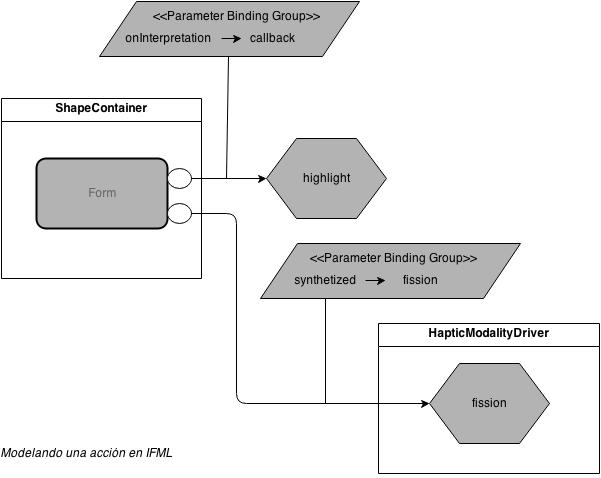
\includegraphics[scale=1,width=\textwidth]{gfx/ifml_example}
    \caption{Modelado de acciones en Shapes App.}
    \label{fig:extension_ifml_example}
  \end{figure}
\end{center}

\section{Aplicaciones Web en la Industria} \label{sec:extension_industria_intro}

La industria ha sido participe en la mencionada ``revolución 2.0''. Negocios como \emph{amazon} crecen considerablemente en esta época y generan necesidades nuevas, lo que motiva a la competencia a imitarlas o superarlas. Con el objetivo de mejorar cualitativamente la aplicaciones desarrolladas y las nuevas, la industria comenzo a generar sus propias herramientas, muchas de ellas \emph{open source}, lo que permitió que otros las usaran, mejorando la calidad general del ecosistema.

Así es como surgen librerías troncales como Backbone.js \citep{ind:backbone}, en el 2010, la cual esta desarrollada íntegramente en JavaScript y ofrece directamente al desarrollador abstracciones para modelos, vistas y controladores desde el lado del cliente, asumiendo del lado del servidor, una API REST. Una librería de este estilo, con un conjunto de dependencias mínimo colaboro directamente con el desarrollo de aplicaciones web ricas, con gran parte de lógica del lado del cliente, capaces de manejar y disparar \emph{in-situ} eventos generados por la misma aplicación o por algún \emph{third-party}. 

Unos años mas tarde, aparecen nuevas herramientas, mas robustas, frameworks, nuevamente desarrollados en JavaScript, destinados a desarrollar la aplicación ''del lado del cliente'', usualmente siguiendo el estilo de backbone.js, consumiendo datos desde algún servicio corriendo del lado del servidor. Entre estos frameworks, se pueden destacar Angular.js de \citep{ind:angular} y Ember.js \citep{ind:ember}. Nuevamente, estas herramientas son \emph{open source} y tienen gran soporte por parte de sus respectivas comunidades, lo que permite retro-alimentar el ecosistema de aplicaciones ricas, haciéndolas perdurar en el tiempo.

Dentro de la industria no hay que dejar de lado a los desarrolladores de navegadores. Grandes empresas como Google, Apple y la fundación Mozilla contribuyen a la mejora de este escenario a través del desarrollo de navegadores que implementen los estándares de la W3C. Esto posibilita el acceso a nuevas capacidades, como por ejemplo la API para WebRTC, la tecnología capaz de brindarle a las aplicaciones la capacidad de acceder a recursos tales como la cámara o el micrófono y compartirlos por internet. También hay que tener en cuenta la relación existente entre la implementación de los estándares y estas grandes compañías, ya que usualmente desarrolladores pertenecientes a las mismas participan en los comités donde se definen estas nuevas APIs. 

\section{Conexión con la Industria} \label{sec:extension_industria_conexion}

Similar al caso anterior, la relación entre las aplicaciones web modernas que se pueden generando utilizando las herramientas que brinda la industria y la plataforma propuesta es de independencia entre ambas. 
La plataforma puede ser consumida desde el contexto de una aplicación web a través del uso de una librería provista. Dicha librería, encapsula una API de acceso a la plataforma y es vista desde la aplicación como una dependencia mas. Con el uso de herramientas como require.js [link], esta dependencia puede ser encapsulada en algún modulo particular de la aplicación web. 

\section{Resumen del Capítulo} \label{sec:extension_conclusion}
Se ha especificado el contexto de aplicación web en el cual la plataforma puede insertarse. Se ha puesto enfasis en analizar este contexto desde dos aristas, el ambito academico y la industria. De esta forma es mas claro ver como se puede utilizar la herramienta desarrollada y como encaja en el escenario actual.

En el siguiente capítulo se mostrará de forma integral el uso de la plataforma por medio del desarrollo de una aplicación web que servira también como modo de \emph{validación por implementación} para la plataforma. % Chapter 4

% Chapter 5 - Desarrollo integral de una aplicación web usando la plataforma plusultra

\chapter{Desarrollo de una aplicaci\'{o}n web multimodal} % Chapter title

\label{ch:demo_development} 
% ### Introducción de capítulo
Los desarrollos de software en la web han avanzado desde sitios estáticos fuertemente orientados al hipertexto, en sus primeros años, a las \textit{aplicaciones} web actuales, similares en robustez y capacidad a las homólogas de escritorio pero con nuevas capacidades típicas del medio, como pueden ser aspectos de programación distribuida o tiempo real. Este avance no ha sido excluyente si no que se han ido añadiendo nuevas capas de funcionalidades. 

La aplicación web introducida en este capítulo tiene el objeto de actuar como herramienta de demostración y validación de la plataforma desarrollada, \emph{Plusultra}. Aunque también añade, a través de un conjunto de tecnologías, una nueva capa de funcionalidad multimodal al dominio de las aplicaciones web.

\section{Introducción} \label{sec:demo_intro}
Dentro del ámbito de una aplicación web, numerosos eventos pueden ocurrir, algunos generados por el usuario otros por la lógica de la aplicación (tanto cliente como servidor). Estos eventos generan en la mayoría de los casos que se dispare una acción y son usualmente acompañados por una animación a modo de feedback visual para darle fuerza al foco de la acción, ayudando a que el usuario mantenga en todo momento una ``imagen'' clara del estado del sistema, \ie~ que el usuario sepa qué ha ocurrido y que está ocurriendo. Pero esta no es la única forma de indicarle y/o darle mas feedback al usuario, existen diferentes vías de comunicación que pueden ser utilizadas con el simple e importante objetivo de brindar mas información y contexto \Eg~ un estado de error es comúnmente transmitido usando el color rojo; es posible agregar otro canal y estimular otro sensor, como puede ser la piel a través de una corta y clara vibración (similar a la que estamos recibimos de los smartphones), logrando así enriquecer la comunicación, cargando la autopista de información usuario-computador.

A través del uso de la plataforma \emph{Plusultra} añadiremos un conjunto de nuevas modalidades al sistema, que generaran nuevos y definidos eventos para que puedan ser capturados dentro del ambiente de una aplicación web. Los usuarios de la misma se beneficiaran de estas nuevas capacidades de interacción, enriqueciendo así a una simple aplicación desarrollada a modo de probar las ventajas que provee el uso de la plataforma.

\subsection{Objetivo}
Desarrollar una aplicación web rica, utilizando un conjunto de dependencias acotado con el fin de hacer énfasis en el uso de la plataforma \emph{Plusultra} y en el agregado de nuevas modalidades dentro de la aplicación.

La aplicación, si bien es de alcance limitado por ser una demostración, tiene el objeto de funcionar dentro del área de entretenimiento. Representa al clásico juego de niños de ``formas'', donde se busca estimular el reconocimiento de patrones. Al hacer encajar las piezas en su lugar, se consigue una retroalimentación que puede verse incluso acompañado de estímulos externos (por parte de los padres, por ejemplo), premiando el éxito, es decir, esta acción de encastrar una pieza en su lugar; todo esto derivando en el conocimiento (y/o refuerzo) de nuevas formas para el niño.

Aquí se traslada este juego a una versión digital del mismo. A través del uso de la plataforma \emph{Plusultra} y un conjunto acotado de modalidades, se extenderán las capacidades de interacción con el fin de generar mas estímulos en el usuario y así incrementar el \emph{feedback} total de la aplicación. 

\subsection{Requerimientos}
Mas allá de los requerimientos iniciales para desarrollar cualquier aplicación, la creación de una aplicación multimodal implica conocer cuáles son y cómo operan los dispositivos de modalidad que vayan a ser usados. 

Para el desarrollo puntual de esta aplicación fueron creados dos \emph{drivers} de modalidad para conectar dos nuevas modalidades, una háptica y otra aero-gestual. 
Estos controladores ofrecen un conjunto de eventos y en algunos casos abren un camino bidireccional entre modalidad y aplicación, es decir, permiten la modificación de parámetros de modalidad en tiempo real. 

Mas adelante se muestran los principales detalles para la creación de un driver de modalidad genérico. 

\subsection{Módulos Principales}

A continuación se describen los principales módulos que componen a la aplicación \emph{shapes}:
\begin{itemize}
\item \texttt{main.js}; representa el contenedor principal de la aplicación, unifica las principales dependencias y dispara el inicio de la aplicación web junto con el panel visor de información de desarrollo.

\item \texttt{visor.js}; contiene la lógica necesaria para brindar información de estado útil para depurar la aplicación durante el desarrollo.

\item \texttt{shapes.js}; coordina los principales eventos de la aplicación, estos pueden ser eventos internos disparados por la aplicación o externos, despachados por alguna de las modalidades. Estos últimos, cuando ocurren son distribuidos a lo largo de todos los clientes conectados a la plataforma.

\item \texttt{interactive.js}; se encarga de administrar de manera uniforme los eventos de drag \& drop que ocurran en la aplicación.

\item \texttt{gyes.js}; es el módulo cliente oficial para conectarse con \emph{Plusultra}. Luego de obtener la llave de acceso a la plataforma, el desarrollador puede comenzar a utilizar un determinado número de instancias de la plataforma. El módulo brinda los principales eventos a los cuales la aplicación puede conectarse y actuar.

\item \texttt{HapticMD}; representa al controlador de modalidad háptico. El mismo esta desarrollado para aprovechar las capacidades de los dispositivos móviles modernos en el ámbito de una aplicación web rica. Provee eventos para definir interacción de entrada a través de gestos táctiles y de salida, a través de feedback vibro-táctiles.

\item \texttt{AirPointerMD}; es el controlador que administra la modalidad aero-gestual, \ie gestos aéreos, utilizando las manos. Este módulo utiliza como dispositivo de hardware al artefacto Leap, lo que permite conseguir información variada sobre manos y dedos sin necesidad de hardware extra \emph{en el} usuario. Este controlador brinda eventos de entrada sobre la posición de alguno de los dedos, el cual será usado como puntero para conseguir una manipulación básica directa sobre los elementos de la aplicación.
\end{itemize}

En la siguiente figura \ref{fig:demo_shapes_app}, se pueden observar a simple vista los principales módulos de la aplicación \emph{shapes}.
% FIGURA DE móduloS SHAPES APP
\begin{center}
  \begin{figure}[h]
    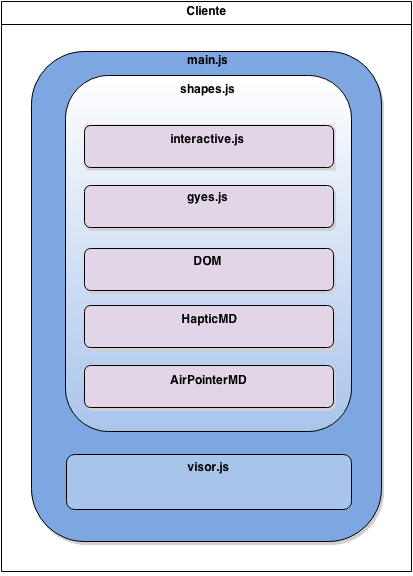
\includegraphics[scale=0.7]{gfx/shapes_app_demo}
    \caption{Módulos de la aplicación web Shapes}
    \label{fig:demo_shapes_app}
  \end{figure}
\end{center}


Los módulos desarrollados para esta aplicación se realizaron usando el patrón \emph{module}, como puede verse en \citet{demo:module_pattern}. A través del uso del mismo se consigue una división de responsabilidades y conocimiento, distinguiendo partes publicas (API) de privadas (implementación). Además permite aplicar una simple pero solida capacidad de manejo de dependencias internas. 

\subsection{Conectando a la Plataforma}
Con el fin de extender el conjunto de modalidades de una aplicación web, se propone la utilización de \emph{Plusultra}. La misma provee un servicio, en tiempo-real, de comunicación con dispositivos de modalidad. En el caso concreto de la aplicación \texttt{Shapes}, se han utilizado dos dispositivos de modalidad, el Leap Motion y los controladores táctiles de los dispositivos móviles. Agregar estas nuevas modalidades aumenta la capacidad de interacción con la aplicación desarrollada. Estas nuevas capacidades pueden ser aprovechadas por el desarrollador de la aplicación web mediante el consumo de los eventos que las mismas generan y que son transmitidos mediante la plataforma. 

En la figura \ref{fig:demo_shapes_app_arq} puede verse la relación entre los componentes arquitectonicos de la aplicación desarrollada:

% FIGURA DE ARQ SHAPES APP
\begin{center}
  \begin{figure}[h]
    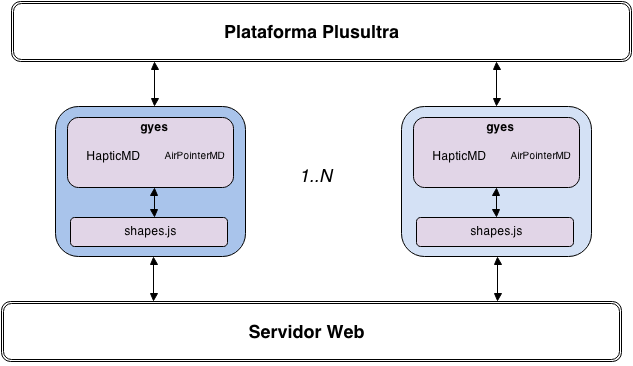
\includegraphics[scale=0.6]{gfx/shapes_app_arq}
    \caption{Vista de la arquitectura de la aplicación Shapes}
    \label{fig:demo_shapes_app_arq}
  \end{figure}
\end{center}


Para conectarse con la plataforma desde el contexto de una aplicación web el desarrollador debe incluir como una dependencia JavaScript, a su entorno de desarrollo, al módulo \texttt{gyes}. Este módulo brinda una interfaz de acceso a la plataforma.

Para conectarse es necesario contar con una llave de acceso y ejecutar el llamado a conexión usando el método \texttt{authenticate}. Este sistema de autenticación es simple y busca emular un escenario ``real''; debería ser mejorado de forma acorde antes de ser llevado a un entorno de producción.

Luego de la autenticación a la plataforma, el desarrollador puede comenzar a utilizar los drivers de modalidad que considere necesarios. Para esta aplicación se utilizan, un driver aero-gestual, denominado \emph{AirPointerMD} y otro, \emph{HapticMD}, usado como controlador háptico. A través del módulo \texttt{gyes} el desarrollador instancia las modalidades dentro de la aplicación web, por ejemplo:

\begin{lstlisting}
    // Construye una nueva modalidad háptica
    var hapticMod = new gyes.Modality( 'webHaptic', 'both', {} ); 
    // Configura algunas opciones del driver como por ej, qu\'{e} gestos hápticos capturar
    var driverOptions = {
      'hapticEvents': [ 'touch, hold' ],
      'element': doc.getElementById('shapes')
    };
    // Construye el driver de modalidad
    var hapticDriver = new HapticMD( driverOptions );
    // Conecta la modalidad con el driver
    hapticMod.use( hapticDriver );
    // Inserta la modalidad en la plataforma.
    _client.addModality( app_key, hapticMod );
\end{lstlisting}

Luego de instanciar y conectar las modalidades deben definirse las interpretaciones necesarias, \ie~ una estructura que da valor semántico a un conjunto de eventos (posiblemente generados por las modalidades) que ocurren en un intervalo de tiempo acotado. Entonces, para que una interpretación ocurra deben generarse determinados eventos en un instante de tiempo, la captura de estos eventos produce una fusión y es tratada por el motor de fusión distribuida del módulo \texttt{gyes}. Un ejemplo donde se muestra como instanciar el motor de fusión es el siguiente:

\begin{lstlisting}
    // El motor de fusión recibe interpretaciones como entrada.
    _gestureInterpretation = new gyes.Interpretation( ['fingerover', 'hold'] );
    // Algunas intepretaciones pueden producir sintetizado de eventos.
    _gestureInterpretation.canSynthetize( hapticMod.name, hapticDriver.getID(), 2000 );

    // Construcción de un motor de fusión.
    _fusion = new gyes.Fusion( {'verbose':true} );
    // Agregando interpretaciones al motor de fusión.
    _fusion.fuse( _gestureInterpretation );
\end{lstlisting}

Finalmente, luego de crear las interpretaciones necesarias junto al motor de fusión distribuida, lo único que queda por hacer es instanciar el sistema de fisión.

A través de este sistema, el desarrollador puede controlar programaticamente qué hacer cuando es detectada alguna interpretación. 

El sistema de fisión, permite conectar una función para que sea llamada de manera asincrónica luego de la ocurrencia de una interpretación, como puede verse a continuación:

\begin{lstlisting}
    // Construye el sistema de fisión
    var _fission = new gyes.Fission();
    
    // Conecta una interpretación con una función anónima.
    _fission.on( _gestureInterpretation.getName(), function(data){
      console.log( 'A new interpretation happened: ', data );
      gestName.textContent = '';
      gestElem.classList.remove( 'highlight' );
      gestDataText.classList.remove( 'invisible' );
      gestDataText.textContent = 'FISION';
      gestData.classList.add( 'highlight' );
      setTimeout(function(){
        gestDataText.classList.add( 'invisible' );
        gestData.classList.remove( 'highlight' );
        gestDataText.textContent = '';
      }, 2000);
    });
\end{lstlisting}

De esta forma se han mostrado los principales puntos de conexión necesarios para utilizar la plataforma \emph{Plusultra} en su primera versión.

\section{Construcción de un Driver de Modalidad}
Para el desarrollo de una aplicación web multimodal es necesario contar con drivers o controladores que den soporte a los dispositivos de modalidad que vayan a ser usados. La plataforma \emph{Plusultra} es agnóstica respecto al dispositivo de modalidad usado, brindando a través del módulo \emph{gyes} una interfaz para conectar un nuevo dispositivo al sistema. Un posible trabajo a futuro y aporte a la plataforma sería la creación de un catálogo online de todos los drivers de modalidad disponibles.

El desarrollo de un nuevo driver de modalidad es una tarea relativamente simple, aunque esto puede variar entre dispositivos. El módulo \emph{gyes} provee una interfaz para la creación de drivers en JavaScript, aunque es posible desarrollar un driver en otro lenguaje, simplemente siguiendo el protocolo (ver sub-sección protocolo \ref{subsection:protocol}), provisto por \emph{Plusultra}.
A continuación se muestran los principales métodos a implementar para crear un driver de modalidad, la conexión del mismo a la plataforma se definió anteriormente.

\begin{lstlisting}
// Incluir el canal de comunicación de gyes.
var ModalityDriverChannel = require( '../gyes/build/gyes' ).ModalityDriver;

// Declaramos el constructor del driver de modalidad. Ej:
module.exports = HapticModalityDriver;

// El constructor generado hereda los eventos a implementar del canal de drivers de modalidad.
inherits( HapticModalityDriver, ModalityDriverChannel );

// Si el dispositivo de modalidad puede sintetizar datos, entonces es posible conectar el evento de sintesis con alguna función interna. Ejemplo del driver háptico:
this.on( 'synthetized', this.fission.bind(this) );

// Si solo necesitamos disparar eventos de "entrada":
this.fire( 'recognized', {'gesture':data.type} );

\end{lstlisting}

Por lo tanto existen dos eventos importantes a tener en cuenta en la realización de un driver de modalidad; el evento para disparar algo ``sensado'' por el dispositivo, etiquetado como \emph{recognized} y el evento para recibir datos de parte de la aplicación y sintetizarlos, denominado \emph{synthetized}.
De esta forma es posible crear un nuevo driver para conectar un nuevo dispositivo al sistema y usarlo en el ámbito de una aplicación web. Es importante destacar que un componente creado de esta manera puede ser compartido y re-utilizado, la única dependencia es contar con el hardware indicado, es decir aquel para el cual fue desarrollado dicho driver. 

Esto permite pensar en la posibilidad de contar con un catalogo de drivers de la plataforma.

\section{Componentes en Acción}
La aplicación Shapes es una prueba de concepto que busca poner en evidencia una interacción multimodal en el navegador. Sumado a esto, la plataforma posibilita la colaboración en tiempo real entre pares. Por lo tanto, es posible contar con mas de un usuario al mismo tiempo y generar entre los usuarios la interacción multimodal. Más aun y debido a la naturaleza distribuida del entorno, la plataforma propaga la señal generada en un evento multimodal de fisión que podrá ser  percibido por todos los clientes (no solo aquellos involucrados en la generación del evento). Esta señal de fisión será recibida en los clientes, los cuales representan un conjunto de hardware heterogéneo, implicando distintas capacidades de afectar al usuario; en el ejemplo aquí presentado, si el usuario esta utilizando la aplicación desde un dispositivo móvil podrá recibir una vibración particular como resultado de una acción multimodal. 

En el siguiente gráfico \ref{fig:demo_show_shapes} se sintetiza el flujo de comunicación habitual de una aplicación web multimodal.

\marginpar{
Referencias: 

\begin{itemize}

\item \textit{Triangulo}: representa a un dispositivo de modalidad.

\end{itemize}}

% FIGURA Flujo de comunicación
\begin{center}
  \begin{figure}[h]
    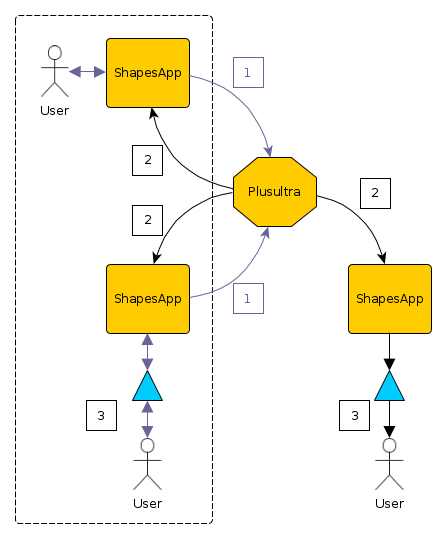
\includegraphics[scale=0.7]{gfx/example_showcase}
    \caption{Flujo de comunicación.}
    \label{fig:demo_show_shapes}
  \end{figure}
\end{center}

Flujo:
\begin{itemize}

\item 1) Parte de un acción multimodal. Distintos clientes están disparando las partes que conforman a una interacción soportada en la aplicación, esto es por ejemplo, depositar una pieza en el lugar correspondiente sumado a seleccionar y mantener la selección de la pieza sobre el contenedor. Esto ocurre localmente y será distribuido por la plataforma.

\item 2) Se realiza la distribución de eventos generados en 1. Esto puede disparar en algunos clientes la interacción multimodal, mas específicamente, una fusión y luego una fisión. Estos eventos son tratados de forma independiente y son propagados por la plataforma. 

\item 3) Si el proceso de fusión genera una fisión, la misma es propagada, esto puede desencadenar alguna acción en la modalidad conectada al cliente.

\end{itemize}

\section{Resumen del Capítulo}
El principal objetivo de la plataforma \emph{Plusultra} es agrandar de manera uniforme el conjunto de modalidades que soportan actualmente las aplicaciones web. Este conjunto  es muy limitado, concentrado en las principales formas de comunicación con el ordenador, como lo son el mouse, el teclado y el feedback visual. En muy pocos casos una aplicación web va mas allá de eso y la principal razón puede estar ubicada en las dificultades propias de la tarea junto a la falta de información al respecto. Yendo un poco mas allá, imaginar el soporte a mas de una modalidad al mismo tiempo, parece difícil de visualizar y por ende de llevar a cabo.

Superar estas cuestiones fueron las premisas constantes durante el desarrollo de la plataforma y a través de la construcción de la aplicación ejemplo \texttt{Shapes} se mostró como es posible crear una aplicación web multimodal con un conjunto acotado y mínimo de  dependencias externas. Si bien existen cuestiones a mejorar, como la simplificación de la API del módulo \texttt{gyes} o las mejoras en el sistema de autenticación con la plataforma, la solución aquí propuesta ha funcionado como un recurso exitoso y concreto al problema de desarrollar una aplicación web multimodal. % Chapter 5

\cleardoublepage % Empty page before the start of the next part

%------------------------------------------------

\ctparttext{El desarrollo de aplicaciones multimodales parece ser el camino a seguir por una parte de la industria. Esto se refleja en el avance en los dispositivos móviles y en diversos proyectos de hardware abierto los cuales ``oxigenan'' las vías de comunicación aun mas.

Profundizar y mantener en órbita estos conceptos se vuelve entonces una estrategia adecuada.} 

\part{Conclusiones y trabajo futuro}

% Chapter 6 - Conclusiones & Trabajo Futuro

\chapter{Conclusiones \& Trabajo Futuro} % Chapter title

\label{ch:end_future} % ### Introducción de capitulo
Conceptos como \emph{Wearable Computing}, \emph{Sensors Fusion} o incluso \emph{Pervasive Computing} han vuelto a ganar impulso recientemente. Utilizando tecnología como placas arduino o similares, implementar pruebas de concepto o prototipos de proyectos de las áreas antes mencionadas, se ha vuelvo mas simple, ya no es necesario contar con conocimientos avanzados de electrónica o saber programar un PIC; estas ventajas reducen las barreras para continuar experimentando en dichas áreas.

Es en este contexto de computación ubicua o ''fuertemente'' móvil es donde es interesante pensar en usar conceptos de desarrollo de aplicaciones multimodales, aprovechando el posible enriquecimiento en las formas de comunicación que estos nuevos ''caminos'' ofrecen para aumentar la experiencia del usuario dentro de la aplicación o incluso para introducir nuevos usuarios gracias a los beneficios conseguidos por la expansión en el conjunto de interacción del sistema.

\marginpar{Sharon Oviatt escribió en 1999 un trabajo donde ataca 10 mitos que suelen generarse alrededor de las aplicaciones multimodales \citep{oviatt1999ten}. Este trabajo resulta aun hoy en dia muy relevante y es una lectura recomendada para todo aquel que se vea frente a la necesidad de comenzar a desarrollar una aplicación multimodal e incluso para el público en general.}
De acuerdo a \citet{kortum2008hci}, los sistemas multimodales dan libertad a los usuarios de elegir como comunicarse con la aplicación, robustez para disminuir errores al tener mas de una modalidad para indicar una acción, \eg el comando <<apuntar aquí>> en una aplicación de información geoespacial, puede ganar precisión utilizando un disparador mediante voz (\emph{''apuntar aquí''}), sumado a un evento sobre una superficie táctil; especialmente si lo comparamos con una aplicación similar que solo cuente con una única modalidad (háptica o por voz) de interacción. Estos sistemas incluso pueden introducir ventajas de rendimiento para determinaras tareas (\eg  visual-espacial), aunque esto depende de la combinación de modalidades. Por ejemplo, en el caso de sistemas que combine gestos (mediante un lapiz optico) con ordenes via voz, resultados han mostrado que se obtiene una mejora del 10\% en los tiempos de terminación de la tarea, se reducen los errores críticos en un 36\% y una reducción del 50\% en problemas de fluidez espontanea, junto a mejoras en las construcción linguisticas, según \citet{oviatt1998referential}.

\section{Conclusiones Sobre el Desarrollo} \label{sec:end_work}
Dentro del marco del presente trabajo de grado, se ha desarrollado una plataforma que permite aumentar el conjunto de canales de interacción de una aplicación web, a través del soporte de interacciones multimodales. Estas nuevas capacidades de interacción pueden ser consumidas en conjunto o por separado, el desarrollador de la aplicación web es quien tiene el control sobre esto. Esta plataforma, en conjunto con el cliente y el protocolo desarrollados, han sido validadas mediante el desarrollo de una aplicación web que no solo permite su uso mediantes los canales clásicos como el teclado y mouse, si no que también es posible interactuar usando el canal háptico y gestual-aéreo. Incluso en el canal haptico se explora la retroalimentación, mediante el uso de motores de vibración. Es decir, el usuario puede \emph{sentir} nuestra aplicación. Todo esto sin perder las características clave de la web, como colaboración, fácil acceso y distribución.

Esta aplicación ha sido desarrollada con los fines de validar la plataforma propuesta y ayudar a mostrar las capacidades de los sistemas multimodales en la web. Por lo tanto constituye una simple demostración del alcance de la herramienta desarrollada. Con mas trabajo y recursos es perfectamente posible generar una experiencia mas rica que incluya, tal vez, a mas dispositivos y canales. 

Teniendo esto en cuenta, los avances aquí propuestos resultan satisfactorios y cumplen con el punto establecido en un principio, extender las capacidades de interacción de las aplicaciones web. La experiencia en general ha resultado satisfactoria y de gran aprendizaje, por ejemplo, en el desarrollo de una aplicación multimodal, uno de los componentes clave es el motor de fusión, en este trabajo se ha desarrollado un nuevo tipo de moto, si bien es bastante simple, cuenta con una característica completamente novedosa, esta distribuido entre los clientes. A través de mas pruebas seria posible saber que tan buena o mala puede ser este nuevo rasgo, en la aplicación a modo de demostración desarrollada, este motor ha sido funcional permitiendo una detección rápida de eventos mientras disminuía la complejidad en el desarrollo del mismo. En la próxima sección se detallan algunas de estas cuestiones, que pueden extenderse como posibles trabajos a futuro.

\section{Trabajo Futuro} \label{sec:end_future}
El desarrollo de un sistema nuevo en un escenario donde antes no existia nada similar de acuerdo a lo visto en el capitulo \ref{ch:estado_arte} supone un desafio. Mas alla de la dificultad per se de llevar a cabo el desarrollo, existen numerosas decisiones que deben ser tomadas con el objetivo de llegar a destino, algunas pueden ser supuestas con antelación y otras simplemente, no pueden serlo, mas aun cuando todo el equipo de trabajo esta constituido en una sola persona. Muchas de estas decisiones se encuentran detalladas en esta sección y pueden ser vistas como posibles mejoras a realizar, otras resultaron en nuevos problemas, que no podian ser tratados en su momento porque hubiesen desviado la atención y el objetivo principal del trabajo, construir la plataforma y aumentar las capacidades de interacción de las aplicaciones web; a las cuales se les ha brindado una solución que puede no ser la mas apropiada, pero que ha servido para cumplir el objetivo propuesto.

\subsection{Performance de los Motores de Fusión y Fisión Distribuidos}
Seria interesante conocer la performance de los motores de fusión y fisión desarrollados. Esto permitiría detectar problemas desconocidos o cuellos de botella de la plataforma. Además de brindar una forma de comparación con otras herramientas similares del mercado. Una posible técnica de medición de performance podría ser la propuesta por \citet{dumas2009benchmarking}. Durante el desarrollo del trabajo se priorizo cumplir con el objetivo de crear la plataforma, para luego de eso, considerar una etapa, en otro trabajo, de medición de performance.

\subsection{Mejoras Especificas al Desarrollo del Motor de Fusión}
Durante la creación del motor de fusión, uno de los momentos clave, fue el desarrollo de la ``ventana'' de captura de eventos. La misma es configurable, en cuanto al tiempo que se encuentra \textit{abierta} y fue construida usando algunas primitivas del lenguaje JavaScript. Construir un sistema de relojes propio, para controlar la apertura de la ventana seria ser una mejora notable al mantenimiento del sistema. También seria importante enriquecer el motor de fusión añadiendo soporte de prioridades entre modalidades, configurable por el desarrollador a su vez como el manejo de orden y no solo simple ocurrencia, de eventos.

\subsection{Mejoras de Usabilidad en la API}
Actualmente, la primer versión de la API del cliente es la que ha sido descripta en el capitulo \ref{ch:enlace}, y vista en uso en el capitulo \ref{ch:demo_development}. La misma puede ser mejorada, ya sea añadiendo nuevos métodos que hagan mas simple la tarea del desarrollador o removiendo o unificando operaciones existentes, con el mismo objetivo. Una manera de detectar estos puntos críticos es involucrando mas desarrolladores que consuman y utilicen la plataforma, teniendo en cuenta el feedback de los mismos en una nueva versión de la API.

\subsection{Consolidar a plusultra como PAAS}
La plataforma desarrollada tiene intenciones de funcionar como una plataforma como servicio (\emph{PAAS}). Es decir, podría convertirse en un producto comercial que brinde la capacidad de desarrollo web multimodal ocultando cuestiones de hardware externas al problema que se desea resolver. Para conseguir esto, algunas cuestiones fueron tenidas en cuenta durante el desarrollo de este trabajo, pero en otras se decidió no llevarlas a cabo, \eg capacidades de autenticación o un servicio web para indicar el desarrollo de una nueva aplicación multimodal.

\subsection{Crear Catalogo de Drivers de Modalidad}
Un aporte significativo para esta plataforma sería la creación de un catalogo de drivers de modalidad, ofrecido como un servicio web. De esta manera, cualquier persona que desee crear una nueva aplicación multimodal podría revisar primero el catalogo para saber si el hardware con el que cuenta tiene soporte. También serviría para impulsar y unificar el desarrollo de los mismos.

\subsection{Crear Aplicaciones Web usando la Plataforma}
Para detectar posibles problemas existentes que han permanecido en silencio o mejorar la usabilidad de la plataforma es importante y beneficioso contar con un ecosistema saludable de aplicaciones y drivers. El equipo de desarrollo detrás de una nueva aplicación multimodal que use la plataforma puede generar una considerable cantidad de feedback que puede ser muy útil.

\section{Enlaces a los Repositorios} \label{sec:end_links}
A continuación se encuentra un listado de enlaces a los repositorios de los componentes de la plataforma:
\begin{itemize}

\item \href{https://github.com/dpaez/plusultra}{Plataforma plusultra.}  (github.com/dpaez/plusultra)

\item \href{https://github.com/dpaez/gyes}{Módulo Interfaz gyes.} (github.com/dpaez/gyes)

\item \href{https://github.com/dpaez/HapticModalityDriver}{Driver de Modalidad háptico.} (github.com/dpaez/HapticModalityDriver)

\item \href{https://github.com/dpaez/AirPointerDriver}{Driver de Modalidad gestual-aéreo.} (github.com/dpaez/AirPointerDriver)

\item \href{https://github.com/dpaez/shapes\_app}{Aplicación Desarrollada usando la Plataforma.} (github.com/dpaez/shapes\_app)

\end{itemize}

\cleardoublepage % Empty page before the start of the next part

%------------------------------------------------

%\ctparttext{A continuación se exponen las características del medio al cual se agregará el soporte para las diferentes modalidades. Luego se esgrimirán los aspectos particulares que esta arquitectura propone y su relación con otras alternativas clásicas.} 


%% Chapter 3 - APIs, enlace con las modalidades

\chapter{Enlace con las modalidades} % Chapter title

\label{ch:enlace} 

%----------------------------------------------------------------------------------------

% ### Introducción de capítulo

 
\section{Arquitectura Propuesta} \label{sec:enlace_overview}
%Primer vistazo general de los ''endpoints'' del sistema, que conectamos? como se consume?
A grandes rasgos, los puntos de entrada a la plataforma \emph{Plusultra} introducida en el capítulo anterior, estarán ubicados en dos lugares diferentes:

\begin{itemize}
\item \textbf{Clientes Web}; aquí también reside la lógica de la aplicación. En conjunto crean una experiencia multimodal en la web. Dentro de los clientes web, podemos encontrar capacidades extra que pueden ser usadas a su vez como modalidades (\ie ~un cliente corriendo en un smartphone puede tener acceso a sensores, que a su vez, pueden ser usados como reconocedores). Mas adelante en este capítulo, se analizará esta situación.
\item \textbf{Dispositivos de modalidad}; se refiere a todos aquellos dispositivos especialmente dedicados a reconocer o sintetizar una modalidad, \eg~ Falcon de Novint o Leap Motion, por mencionar algunos.
\end{itemize}

Para conectar estos puntos de entrada, se construyo un modulo de acceso que puede ser consumido por igual tanto del lado del cliente como del servidor o \emph{standalone} (dispositivos de modalidad). Ademas se ha desarrollado una primera versión de un protocolo de comunicación que acompaña dicha interfaz de comunicación. Este protocolo abre el camino a otros desarrolladores para que puedan diseñar soluciones utilizando diferentes lenguajes. 
En el mismo se describe los mensajes utilizados para un enlace efectivo con la plataforma \emph{Plusultra}. De esta manera, siguiendo a este protocolo versionado, la API puede portarse a otros lenguajes de programación extendiendo así el alcance y uso de la plataforma.

\subsection{Modulo Híbrido Cliente/Servidor}
Prácticamente todo el desarrollo de este trabajo se ha llevado a cabo utilizando el lenguaje JavaScript. Dado que se busca expandir la capacidad actual de comunicación de las aplicaciones web, es lógico basar la mayor parte de la base de código en dicho lenguaje. Usando la plataforma Node.js, es posible correr JavaScript del lado del servidor también, haciéndolo ubicuo en múltiples escenarios. Teniendo en cuenta estas capacidades, se decidió desarrollar un modulo que pueda aprovechar estos aspectos y ser de utilidad en diversas circunstancias o casos de uso.
 
De esta forma se introduce el módulo \emph{Gyes}. A través de este componente es posible conectarse al sistema, transmitir datos de modalidades, crear nuevas modalidades, crear interpretaciones, capturar salidas del sistema de fisión; por nombrar los casos mas importantes. 

\subsection{Vista General}
%Grafico que muestre los componentes introducidos antes y las nuevas interfaces.
El modulo \emph{Gyes} permite realizar diferentes tareas, las cuales tienen como finalidad interactuar con la plataforma \emph{Plusultra} y por consiguiente con el resto de los actores de la aplicación, es decir, con el contexto entero de la aplicación web.
El siguiente gráfico \ref{fig:arq_ours_gyes_action} simplifica una de las principales actividades, utilizar una modalidad como reconocedora de algún tipo de señal para luego propagarla en la aplicación, mediante la plataforma. 

% FIGURA DE GYES en accion
\begin{center}
  \begin{figure}[h]
    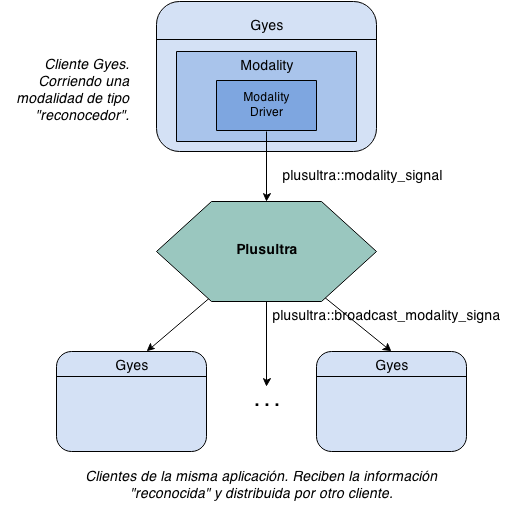
\includegraphics[scale=0.7]{gfx/gyes_action}
    \caption{Modulo Gyes en acción: transmitiendo señales}
    \label{fig:arq_ours_gyes_action}
  \end{figure}
\end{center}

\section{Descripción de la Interfaz del Modulo} \label{sec:enlace_api}
% detalles de la interfaz
En la figura \ref{fig:arq_ours_gyes} se observa de manera directa los principales componentes del modulo de acceso al sistema. Luego extenderemos esta visión a la interacción que ocurre con la plataforma.
A continuación se describirán las interfaces de los componentes junto a una breve introducción a la primer version del protocolo de comunicación entre \emph{Plusultra} y \emph{Gyes}.

% FIGURA DE COMPONENTES GYES
\begin{center}
  \begin{figure}[h]
    \centering
    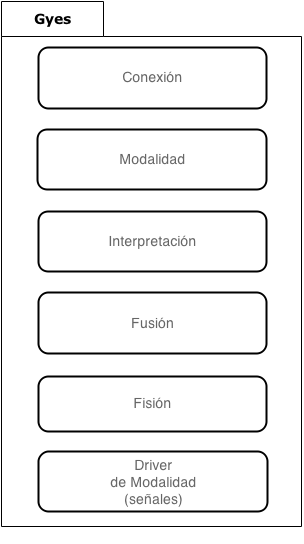
\includegraphics[scale=0.7]{gfx/gyes}
    \caption{Principales componentes del modulo Gyes}
    \label{fig:arq_ours_gyes}
  \end{figure}
\end{center}

\subsection{Componente de Conexión}

Es el componente principal. Desde aquí no solo accedemos a la plataforma si no también al resto de los componentes. 

La función principal es proveer una forma de conectar, tanto para modalidades como clientes a \emph{Plusultra}.
\\

\underline{\textsf{Constructor:}}\\
\begin{lstlisting}
Gyes( appKey, uri, opts )
\end{lstlisting}
Crea una nueva instancia del módulo \emph{Gyes}. Automáticamente inicia una conexión con la plataforma \emph{Plusultra}. 

\underline{\textsf{Principales métodos:}}\\
\begin{itemize}
\item[]
\begin{lstlisting}
gyes::authenticate( appKey )
\end{lstlisting}
Una vez creada la instancia, necesitamos autenticar nuestra aplicación. Para eso el desarrollador web debe contar con una llave, previamente generada, por ejemplo usando algún servicio donde registre la aplicación y la cantidad de instancias a consumir de la plataforma.
\\

\emph{Plusultra} es una plataforma que ha sido diseñada para ser fácilmente escalable a un modelo de PAAS (\emph{Platform as a Service}), de esta forma, múltiples instancias del módulo de plataforma pueden servir a diferentes aplicaciones. Por eso es necesario que cada aplicación posea una llave que la distinga.

\item[]
\begin{lstlisting}
gyes::addModality( aModality )
\end{lstlisting}
Permite agregar una nueva modalidad al sistema. Esto es útil para indicar que determinado cliente cuenta con una modalidad particular la cual, al estar ``agregada'' a la plataforma, puede compartir la información que genera.
\end{itemize}

\subsection{Componente de Modalidad}
%diagrama de secuencia, conexion, fusion/fision

Este módulo permite crear y agregar nuevas modalidades al sistema. Dada la naturaleza variada de las mismas, se decidió separar comportamiento de representación/identificación. El comportamiento esta definido por los drivers, aquí especificamos una representación. Dentro de una aplicación, pueden conectarse mas de una modalidad y por ahora, una modalidad puede usar un driver.
\\

\underline{\textsf{Constructor:}}\\
\begin{lstlisting}
Gyes::Modality( name, type, opts )
\end{lstlisting}
Permite crear un nuevo objeto que representa a una modalidad, la cual podrá ser agregada al sistema. Recibe un nombre (\emph{name}), tipo (\emph{type}), de acuerdo a si es de entrada/salida o ambos y luego opciones (\emph{opts}) particulares para compatibilidad a futuro.
\\

\underline{\textsf{Principales Métodos:}}\\
\begin{itemize}
\item[]
\begin{lstlisting}
modality::use( modalityDriver )
\end{lstlisting}
Conecta una instancia de modalidad con una instancia de driver.
\end{itemize}

\subsection{Componente de Fusión Distribuida}

Permite controlar el motor de fusión de manera programable. Este componente captura \emph{señales} que pueden ser generadas por modalidades o por eventos de la aplicación.
\\

\underline{\textsf{Constructor:}}\\
\begin{lstlisting}
Gyes::Fusion( opts )
\end{lstlisting}
Genera una nueva instancia del motor de fusión. 
\\

\underline{\textsf{Principales métodos:}}\\
\begin{itemize}
\item[]
\begin{lstlisting}
fusion::fuse( anInterpretation )
\end{lstlisting}
Detecta un determinado conjunto de señales, definidos por una interpretación. Cuando dicha interpretación ocurre, puede distribuir esta información entre todos los clientes y comenzar el proceso de activar al sistema de fisión.
\\

La captura de señales se produce manteniendo una ventana de tiempo, donde la misma se actualiza (extiende) cada vez que ocurre un evento que pertenezca a una interpretación. Esto ocurre de forma independiente y distribuida entre todos de la aplicación. Es decir, cada uno cuenta con un motor de fusión. Para que esto funcione, las señales deben ser distribuidas, usando la plataforma, en tiempo real.
\end{itemize}

\subsection{Componente de Fisión Distribuida}

Brinda acceso al sistema de fisión. El desarrollador web, encuentra en este componente un ``punto de salida'' de la plataforma, donde puede conectar la lógica de la aplicación web mientras consume información generada por las distintas señales que recorren el sistema.
\\

\underline{\textsf{Constructor:}}\\
\begin{lstlisting}
Gyes::Fission( opts )
\end{lstlisting}
Genera una nueva instancia del motor de fisión.
\\

\underline{\textsf{Principales Métodos:}}\\
\begin{itemize}
\item[]
\begin{lstlisting}
fission::on( interpretationName, callbackFn )
\end{lstlisting}
El sistema de fisión permite al desarrollador conectar la ocurrencia, asincrónica, de una interpretación con código que afecte a la lógica de negocios de la aplicación.
\end{itemize}

\subsection{Componente de Interpretación}

En los componentes anteriores se menciono el concepto de \emph{interpretación}, aquí se muestra su interfaz y lo que representa.

Este componente permite agrupar un conjunto determinado de señales en un único objeto.
Una interpretación puede representar la conjunción de diferentes modalidades en un único evento.
Las interpretaciones son usadas por el motor de fusión para detectar la ocurrencia de dichas señales e interpretarlas como un único evento alertando al resto de los componentes del sistema sobre dicha ocurrencia.
\\

\underline{\textsf{Constructor:}}
\begin{lstlisting}
Gyes::Interpretation( eventsList )
\end{lstlisting}
Genera una nueva instancia de interpretación. Recibe una lista de señales la cual servirá para organizar al sistema de fusión en el escaneo y detección de ocurrencias de interpretaciones.
\\

\underline{\textsf{Principales Métodos:}}\\
\begin{itemize}
\item[]
\begin{lstlisting}
interpretation::getName()
\end{lstlisting}
Regresa una identificación única para la interpretación. Útil para ``escuchar'' por una determinada ocurrencia.

\item[]
\begin{lstlisting}
interpretation::canSynthetize( modalityID,modalityDriverID,param )
\end{lstlisting}
Permite activar desde la lógica de la aplicación alguna capacidad de sintetizado provista por algún driver de modalidad. Recibe un identificador de modalidad (\emph{modalityID}), un identificador de driver de modalidad (\emph{modalityDriverID}) y parámetros (\emph{params}) opcionales para la función de sintetizado.

\end{itemize}

\subsection{Componente de Driver de Modalidad}

Brinda una interfaz para el desarrollo de diferentes comportamientos sobre una modalidad. Esto permite que la plataforma sea agnóstica a una determinada modalidad particular. A través del uso de señales, el desarrollador de driver de modalidad, podrá escribir la lógica necesaria para su dispositivo de modalidad, ya sea un \emph{reconocedor}, \emph{sintetizador} o de ambos tipos; y conectar esa lógica de forma uniforme a la plataforma.
\\

\underline{\textsf{Constructor:}}\\
\begin{lstlisting}
Gyes::ModalityDriver()
\end{lstlisting}
Genera una instancia que contiene las diferentes señales para conectarse con el cliente y así con la plataforma.
\\

\underline{\textsf{Principales Métodos:}}\\
\begin{itemize}
\item[]
\begin{lstlisting}
modalityDriver::on( signal, callbackFn )
\end{lstlisting}
Permite al desarrollador de driver de modalidad, conectar de forma clara una señal de sintetizado (\emph{synthetized}) o actualización (\emph{updated}) con funcionalidad propia del driver.
\item[]
\begin{lstlisting}
modalityDriver::fire( signal, data )
\end{lstlisting}
Permite disparar una señal de reconocimiento (\emph{recognized}), acompañado de datos producidos por la modalidad. Esta información sera distribuida mediante la plataforma.
\end{itemize}

\subsection{Descripción del Protocolo} \label{subsection:protocol}
Se definió un protocolo de comunicación entre la plataforma y los múltiples clientes \emph{Gyes}. El mismo permite expresar los conceptos definidos durante el trabajo. Estos son: modalidades, señales e interpretaciones. Se utilizo la notación JSON para definirlo.

A través del uso del protocolo podrían crearse clientes en otros lenguajes, que serian capaces de interactuar de igual forma con la plataforma que el cliente Gyes aquí propuesto (desarrollado en JavaScript). 

A continuación se detallan los eventos que conforman el protocolo en la versión 1.

\begin{center}
    \begin{tabular}{| l | l |}
    \hline
    ID & PARÁMETROS:TIPO \\ \hline
    plusultra::authenticate & appKey:string \\ \hline
    plusultra::welcome & - - - \\ \hline
    plusultra::new\_modality & modality:object \\ \hline
    plusultra::broadcast\_new\_modality & modality:object\\ \hline
    plusultra::modality\_signal & signal:object \\ \hline
    plusultra::broadcast\_modality\_signal & signal:object \\ \hline
    plusultra::interpretation & interpretation:object \\ \hline
    plusultra::broadcast\_interpretation & interpretation:object \\
    \hline
    \end{tabular}
\end{center}

\section{Cuestiones Importantes}
Tener a los módulos de fusión y fisión \emph{distribuidos}, es un acercamiento que plantea desafíos.

En primer lugar, cualquier aplicación distribuida gana mayor poder de computo de forma mucha mas ``económica'' ante una variante centralizada. Luego, la decisión de hacer esta solución \emph{distribuida}, esta relacionada directamente con la arquitectura de bajo nivel del ambiente, es decir, la web. Por lo tanto, el acercamiento \emph{per se} no fue forzado, esto dejo lugar a poder ver claramente como podían desarrollarse los aspectos propios del problema, \ie los diferentes componentes que hacen a una aplicación multimodal. Para ello, se partió de la definición clásica de  \citet{dumas2009multimodal}. 

Allí se identificaron los principales componentes a exportar dentro de esta solución. En particular se descartaron, o no se implementaron directamente, el sistema de administración de dialogo (\emph{Dialog Management}) y el sistema de manejo de contexto/historia del usuario (\emph{Context User Model History}). La decisión se basa en que estos componentes pueden ser mantenidos indirectamente en la lógica de la aplicación web, de acuerdo a la necesidad del desarrollador; además la ausencia de estos componentes de forma directa, facilita la transición hacia un modelo distribuido ya que presentan características de aplicación centralizada, \ie~ no hace necesidad de un servicio externo manteniendo esta información.

De todas formas, se mantiene abierto el análisis, específicamente al componente de administración de dialogo, si se detecta alguna manera concreta en la que pueda mejorar la calidad de uso de la herramienta en general.

Si bien, un sistema multimodal con componentes de fusión y fisión distribuidos, puede generar demasiados mensajes y estos pueden afectar su performance general, la solución propuesta esta diseñada para ser escalable, añadiendo mas instancias de \emph{Plusultra} que a su vez puedan manejar mas volumen de mensajes en el tiempo. 

Uno de los aspectos que inicialmente se agrego como distribuido y luego de algunas pruebas se determino que sea mantenido localmente, fue el componente de modalidad. En un principio, al agregar una modalidad a la plataforma, mediante el cliente \emph{Gyes}, la misma era transmitida a todos los demás clientes web. Esto generaba un problema al momento de disparar una interpretación, ya que la misma podía tener asociada una capacidad de sintetizado y si se intentaba activar dicha capacidad en la modalidad recibida por la plataforma, podría ocurrir un error o en un caso silencioso, un gasto de mensajería en vano.
La clave de la plataforma se encuentra en los mensajes que distribuye, estos son: señales de modalidad e interpretaciones (conjunto de señales agrupadas bajo algún valor lógico). Cualquier otro mensaje a ser distribuido puede añadir valor agregado con un costo que debe ser tenido en cuenta porque añade mas mensajería a una plataforma en tiempo real, lo cual puede repercutir directamente en su performance. 

\section{Resumen del Capítulo} \label{sec:enlace_summary}
En el presente capítulo se termino de introducir a los principales actores de la arquitectura de la solución propuesta. En particular, se han descrito aquí a aquellos relacionados a los puntos de entrada/salida del sistema. Estos componentes, en su mayoría, tienen algún tipo de relación con la lógica de la aplicación web donde sean usados; o con la modalidad que se desee integrar al sistema. 

Particularmente, se ha incluido el módulo multiuso \emph{Gyes}, el cual representa una solución tanto para el browser como \emph{standalone}. También se agrega la primer version del protocolo de comunicación entre el cliente y la plataforma, con el fin de dejar abierta una puerta para el desarrollo de otros clientes en diferentes lenguajes. Finalmente se destacan algunos puntos característicos de esta solución distribuida. Mas investigación en este punto puede ocurrir en el futuro, con el desarrollo de mas y variadas aplicaciones que consuman esta plataforma. % Chapter 3

%\cleardoublepage % Empty page before the start of the next part

%----------------------------------------------------------------------------------------
%	THESIS CONTENT - APPENDICES
%----------------------------------------------------------------------------------------

\appendix

\ctparttext{Hasta ahora hemos visto una serie de componentes, que agrupados, son capaces de dar soporte a interacciones multimodales en aplicaciones web. Pero nada se ha especificado sobre alguna modalidad concreta. Aquí se introducirá un primer acercamiento a dos modalidades, para las cuales se han desarrollado sus correspondientes drivers. Se trata de las modalidades háptica y aéreo-gestual.} 

\part{Apéndice} % New part of the thesis for the appendix
% Apéndice - Modalidad Háptica

\chapter{Modalidad H\'{a}ptica} % Chapter title

\label{ch:mod_haptic} 

%----------------------------------------------------------------------------------------
% ### Introducción de capítulo
La modalidad háptica es la que permite la interacción con el órgano mas grande del cuerpo humano, la piel. Particularmente, el sentido del tacto. Este sentido, junto a la vista, permiten, por ejemplo, el rápido reconocimiento de escenarios, percibiendo profundidad y distancias estimadas con los elementos del ambiente así como también una referencia centrada en el usuario, \ie desde mi lugar donde están los elementos.
Una de las principales características del sentido del tacto, es que brinda una autopista directa al sistema nervioso, a través de su propio canal. Esto representa una ventaja con respecto a otros sentidos, como por ejemplo, vista y oído, ya que no requiere un procesamiento (reconocimiento de patrones) previo. Por otro lado, esto indica que la información obtenida por este canal es de mas bajo nivel o mas ``cruda'' y seguramente seran necesarias tareas de filtrado o adaptación de la entrada.



\section{Sentidos Involucrados}
El principal sentido afectado por esta modalidad es el del tacto. A través de este sentido, se pueden identificar dos interfaces, una cutánea y otra cinestésica. La primera se relaciona directamente con la piel y sus diferentes terminales sensitivas, la segunda, en cambio, con músculos y tendones y representa información sobre la ubicación espacial de todo nuestro cuerpo en el ambiente. Ambos canales proporcionan diferente \emph{feedback} al usuario y deberán ser capturados/sintetizados usando diferente hardware, \ie display táctil vs. display cinestésico. Ambos pueden trabajar en conjunto y a diferencia de otros sentidos, el tacto, permite una comunicación bidireccional entre usuario y sistema, de esta forma, se nota claramente que mediante el uso de este canal es posible aumentar claramente la experiencia de usuario, ya que se aumenta el \emph{feedback}. Una posible forma de distinguir estas interfaces, es en cuanto al caudal de información que intentemos enviar por el canal, \ie si solo necesitamos transmitir una alerta para corregir una acción vs. si deseamos transmitir información espacial al usuario; la primera puede ser solucionada usando la interfaz táctil y la segunda la cinestésica.

Existen diferentes formas de estimular el sentido del tacto, los receptores hápticos del cuerpo humano son de tres tipos: mecano-receptores (actúan de acuerdo a la fuerza o presión), termo-receptores (estimulados por la temperatura que reciben) y nociceptores (estimulados por el dolor).
Los sistemas mecano-receptores son los mas populares, y se pueden clasificar en cuatro diferentes sensaciones: presión, tacto, vibración y cosquilleo. La distribución de estos sensores no es uniforme en todo el cuerpo, por lo que aplicar una mecano-estimulación impactara de manera diferente de acuerdo al lugar de acción. Es una cuestión a tener en cuenta antes de desarrollar cualquier tipo de aplicación multimodal que planee utilizar este sentido. En el trabajo de \citet{hale2004deriving}, se clasifican y recomiendan distintas interfaces hápticas, siendo una guia importante al momento de desarrollar una interfaz que consuma esta modalidad.

\section{Interfaces Populares}
Algunas interfaces populares para esta modalidad son el dispositivo Falcon de \href{http://www.novint.com/index.php/novintfalcon}{Novint} o \href{http://www.dentsable.com/haptic-phantom-desktop.htm}{PHANTOM}, ambos de características similares, operan sobre la interfaz táctil brindando un punto de conocimiento al usuario, que mediante el uso del dispositivo puede enviar información aplicando presión y recibir un estimulo, mediante un sistema de motores de vibración. Dispositivos de este estilo, permiten reconocer texturas o ambientes a través de dicha estimulación viéndose limitados a un único punto de contacto, es decir no transmiten información masivamente a todo el cuerpo.

% FIGURA DE MODALIDAD HAPTICA
\begin{center}
  \begin{figure}[h]
    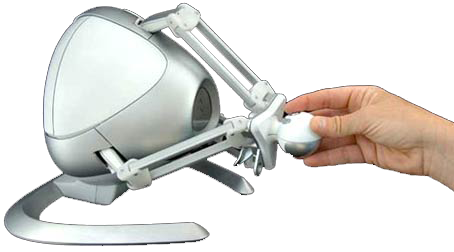
\includegraphics[scale=1,width=\textwidth]{gfx/novint1xe6}
    \caption{Dispositivo Falcon de la compañia Novint}
    \label{fig:apx_novint}
  \end{figure}
\end{center}

Es interesante destacar también la ocurrencia de estimuladores háptico es dispositivos de uso masivo como son los dispositivos móviles o smartphones y también, en los sistemas de entretenimiento, presentes en los joysticks, desde hace bastante tiempo. La interfaz con la que estos dispositivos interactúan es nuevamente la táctil, a través de un sistema de estímulos hacia el usuario, la intención común es brindar algún tipo de alerta sobre alguna acción a realizar.
La presencia de esta modalidad en dispositivos masivos fue una de las características que motivo a que sea una de las primeras modalidades en ser soportadas por la plataforma mediante el desarrollo de un driver.
Existen mas implementaciones de interfaces hápticas que las que se mencionan aquí, para mas información se recomienda ver el capítulo sobre la modalidad háptico de \citet{kortum2008hci}.

\section{Tecnología Utilizada}
En este trabajo se incluye un driver de modalidad que trabaja con displays táctiles y feedback vibro-táctil, por lo que se hará foco en la modalidad de trabajo de los mecano-receptores.
Para aprovechar la ocurrencia masiva de dispositivos vibro-táctiles e interfaces ''touch'', se decidió que el driver utilice el hardware incluido en los móviles, accediendo a los mismos a través de las interfaces estándar HTML5 correspondientes, \eg  \href{http://www.w3.org/TR/vibration/}{API de vibración}.
 % Modalidad háptica
% Apéndice - Modalidad Aero-gestual

\chapter{Modalidad Aero-Gestual} % Chapter title

\label{ch:mod_air} 
Esta modalidad debe ser catalogada inicialmente, dentro del grupo superior de las interfaces gestuales. 
\marginpar{Por interfaces gestuales se hace referencia a aquellas que utilizan movimientos del cuerpo y rostro como señales, que pueden acompañar a la comunicación verbal. En el contexto HCI, el uso de dichas interfaces implica, a través de cámaras o sensores diversos, capturar estos gestos y hacerlos útiles dentro de alguna aplicación.}
En el uso cotidiano que le damos a los gestos, estos suelen complementar la comunicación verbal y son producidos mediante el uso del cuerpo y el rostro. Por esta razón es que esta modalidad tiende a ser usada fácilmente como complemento de otras, \ie~ interfaz de voz.
Una de las ventajas que trae consigo esta interfaz es la universalidad de los gestos en muchos casos, cuando esto ocurre es porque contamos con gestos auto-definidos que rompen las barreras del idioma.

Usualmente encontramos interfaces gestuales en los \emph{pads} de las computadoras portátiles. Un buen ejemplo es el pad de las \emph{ultrabooks}, ya que es común encontrar soporte de numerosos gestos que podemos realizar usando uno o mas dedos.
Al momento de desarrollar cualquier interfaz, si consideramos incluir gestos en la misma, la premisa no debe ser simplemente incluirlos, si no, que tengan un objetivo propio y claro dentro del sistema. 

Uno de los propósitos mas comunes cuando se utilizan interfaces gestuales es el de brindar una forma de trabajo mas ``natural'' al usuario, eliminando cualquier necesidad de hardware extra para interactuar con el sistema, incluso permitiéndole enviar ordenes usando gestos populares, evitando la necesidad de aprender un lenguaje nuevo.

\section{Sentidos Involucrados}
Cuando se habla de gestos, el principal sentido involucrado es el de la visión. Como en muchos otros casos, a través de la vista, recibimos un patrón que cerebro puede detectar muchas veces gracias a nuestro bagaje cultural, aunque en otros casos puede darse que el individuo aprenda un conjunto de gestos nuevos para interactuar con el sistema.

Esta modalidad es de una sola vía, es decir, es un canal de entrada al sistema que no podemos retro-estimular directamente (es posible estimular a otros sentidos como respuesta a un gesto, pero esto es otra cuestión).
Por este motivo y como se menciono anteriormente, esta modalidad suele trabajar en conjunto con otras modalidades en sistemas multimodales, muchas veces funcionando como una herramienta para eliminar ambigüedad introducida por otras interfaces.
 
Los gestos pueden ser clasificados de tres maneras:
\begin{itemize}
\item Semántica; gestos auto-contenidos, comúnmente usados en comunicación no-verbal.
\item Funcional; relacionados al contexto de una aplicación, suelen indicar directivas o comandos, \eg manipulación directa de un elemento.
\item Descriptiva; se concentra en \emph{como} el gesto es realizado.
\end{itemize}

Finalmente, es necesario tener en cuenta la distancia requerida para realizar e interpretar correctamente el gesto, ya que la misma impacta contra el \textit{vocabulario} de gestos a utilizar. Por ejemplo, no es la misma la interacción que podemos tener con una persona frente a frente que si estamos a varios metros de distancia, el conjunto de gestos que usamos cambia. Este es un factor a tener en cuenta cuando se diseña una interfaz gestual.

Particularmente en este trabajo, se hace referencia a interfaces aéreo-gestuales, es decir aquellas que no necesitan de una interfaz externa, como puede ser un dispositivo táctil, para ser usadas; tampoco es necesario que el usuario se acerque a alguna pantalla (aunque esto depende del vocabulario gestual a utilizar). Estas interfaces tienden a usar muy poco o ningún hardware extra, mas allá del dispositivo de escaneo, esto les permite funcionar mas ``naturalmente'', \ie sin necesidad de nada extra en el usuario, posibilitando incluso la captura de gestos conscientes o inconscientes en el usuario.

\section{Interfaces Populares}
Algunas interfaces utilizan técnicas de visión por computadora para detectar los gestos  relevantes del sistema. El trabajo de \citet{wang2009real} es un excelente ejemplo de una técnica efectiva para \emph{trackear}, en este caso, las manos y usarlas como un sistema de gestos funcional, realizando tareas que incluyan manipulación directa con algún elemento de nuestro sistema. 

Otra interfaz que permite capturar información gestual sin necesidad de hardware extra \emph{en el} usuario es el dispositivo \href{https://www.leapmotion.com/}{ Leap Motion}. El mismo utiliza sensores infrarrojos para detectar las manos y triangular posición en tiempo real.
Finalmente, otros dispositivos, populares en sistemas de entretenimiento como son \href{http://www.xbox.com/es-ES/Kinect}{ Kinect, de Microsoft} y \href{http://www.nintendo.com/es_LA/wiiu}{ Wii U de Nintendo}, permiten detectar gestos a nivel cuerpo y a una distancia de un par de metros, generando experiencias de inmersión dentro de los juegos, \emph{trackeando} información gestual del esqueleto humano.

\section{Tecnología Utilizada}
Para este trabajo, se utilizo el dispositivo \textbf{Leap Motion} como herramienta para capturar y acceder a la modalidad aéreo-gestual. Para esto se desarrollo un driver que captura información de uno de los dedos de las manos y la entrega al sistema como si fuera puntero, permitiendo al usuario interactuar de manera funcional con los objetos de la aplicación.

En la figura \ref{fig:apx_airgesture} se puede observar la representación un gesto que puede ser capturado por algún reconocedor, como el mencionado Leap Motion o incluso una cámara web. Este gesto se convierte en una entrada para el sistema que podemos aprovechar, utilizando la plataforma \emph{plusultra}, en el contexto de una aplicación web.

% FIGURA DE MODALIDAD AERO GESTUAL 
\begin{center}
  \begin{figure}[h]
    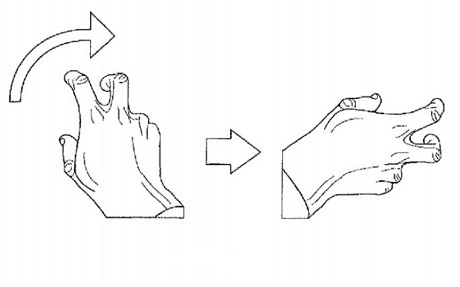
\includegraphics[scale=1,width=\textwidth]{gfx/air-gestures}
    \caption{Representación de un gesto aereo.}
    \label{fig:apx_airgesture}
  \end{figure}
\end{center}
 % Modalidad gestual

%\include{Chapters/Chapter0B} % Appendix B - empty template

%----------------------------------------------------------------------------------------
%	POST-CONTENT THESIS PAGES
%----------------------------------------------------------------------------------------

\cleardoublepage%----------------------------------------------------------------------------------------
%	List of Figures
%----------------------------------------------------------------------------------------

%\refstepcounter{dummy}
\manualmark
\markboth{\spacedlowsmallcaps{\listfigurename}}{\spacedlowsmallcaps{\listfigurename}} 
\refstepcounter{dummy}

\addtocontents{toc}{\protect\vspace{\beforebibskip}} % Place the bibliography slightly below the rest of the document content in the table of contents
\addcontentsline{toc}{chapter}{\tocEntry{\listfigurename}}

%\addcontentsline{toc}{chapter}{\listfigurename} % Uncomment if you would like the list of figures to appear in the table of contents
\pdfbookmark[1]{\listfigurename}{lof} % Bookmark name visible in a PDF viewer
%
\listoffigures
%
\vspace*{8ex}
\newpage % Bibliography

\cleardoublepage% Bibliography

\label{app:bibliography} % Reference the bibliography elsewhere with \autoref{app:bibliography}

\manualmark
\markboth{\spacedlowsmallcaps{\bibname}}{\spacedlowsmallcaps{\bibname}} 
\refstepcounter{dummy}

\addtocontents{toc}{\protect\vspace{\beforebibskip}} % Place the bibliography slightly below the rest of the document content in the table of contents
\addcontentsline{toc}{chapter}{\tocEntry{\bibname}}

\bibliographystyle{plainnat}
%\bibliographystyle{babplain}

\bibliography{Bibliography} % Bibliography

\cleardoublepage% Colophon (a brief description of publication or production notes relevant to the edition)

\pagestyle{empty}

\hfill

\vfill

\pdfbookmark[0]{Colophon}{colophon}

\section*{Colophon}

This document was typeset using the typographical look-and-feel \texttt{classicthesis} developed by Andr\'e Miede. The style was inspired by Robert Bringhurst's seminal book on typography ``\emph{The Elements of Typographic Style}''. \texttt{classicthesis} is available for both \LaTeX\ and \mLyX: 

\begin{center}
\url{http://code.google.com/p/classicthesis/}
\end{center}

\noindent Happy users of \texttt{classicthesis} usually send a real postcard to the author, a collection of postcards received so far is featured here: 

\begin{center}
\url{http://postcards.miede.de/}
\end{center}
 
\bigskip

\noindent\finalVersionString % Colophon

%\cleardoublepage% Declaration

\refstepcounter{dummy}
\pdfbookmark[0]{Declaración}{declaración} % Bookmark name visible in a PDF viewer

\chapter*{Declaración} % Declaration section text

\thispagestyle{empty}

Put your declaration here.
\bigskip
 
\noindent\textit{\myLocation, \myTime}

\smallskip

\begin{flushright}
\begin{tabular}{m{5cm}}
\\ \hline
\centering\myName, \today \\
\end{tabular}
\end{flushright}
 % Declaration

%----------------------------------------------------------------------------------------

\end{document}
